\chapter{Pruebas y resultados}
\section{Introducción}
\label{cap:resultados}

Se reportan los resultados de la línea base (\eegnet{}) y de las tres arquitecturas
objetivo: el Conformer, el modelo fundacional LaBraM (variante Base) y EEGMamba. Con la media
de tres semillas, el protocolo \loso{} supera al intra-sujeto en las cuatro arquitecturas,
\eegnet{}, el Conformer y LaBraM son equivalentes entre sí dentro de $\pm 0.03$ y solo LaBraM
muestra una degradación significativa ante participantes no vistos. Después se informan tres
grupos de variantes sobre la misma base: preprocesamiento y aumentación en el protocolo
intra-sujeto (subsección~\ref{sec:ablaciones-f4}), alineamiento euclidiano y reflexión de canales
en \loso{} (subsección~\ref{sec:f6f8}) y calibración con pocos ensayos del sujeto no visto
(subsección~\ref{sec:fewshot}). Sus condiciones de lectura están en la
subsección~\ref{sec:condiciones-variantes}.



Las cuatro pruebas examinaron la generalización entre personas (Prueba 1), las variantes de procesamiento y calibración (Prueba 2), la transferencia entre conjuntos (Prueba 3) y los criterios adicionales al desempeño (Prueba 4). En conjunto aportaron evidencia para el objetivo~\ref{oe:4}; la segunda examinó el procesamiento del objetivo~\ref{oe:2}, y la primera y la cuarta evaluaron los modelos del objetivo~\ref{oe:3}.

\section{Descripción del conjunto de datos}
\openbmi{} \cite{lee2019} aportó 54 participantes y dos clases de imaginación de movimiento de mano izquierda y derecha, con 400 ensayos por persona, distribuidos en dos sesiones. En cada sesión intra-sujeto se reservaron 20 ensayos para prueba, 144 para entrenamiento y 36 para validación en cada partición estratificada. En \loso{}, 51 sujetos entrenaron, dos validaron y uno se reservó para prueba. Para la evaluación con sujetos apartados se separaron 44 participantes de 10 de prueba. La transferencia empleó WBCIC-SHU \cite{yang2025wbcic}, con 51 participantes y las mismas clases, usando la primera sesión y los 45 canales comunes. Las características y el reparto completo figuran en el capítulo~\ref{cap:metodologia-datos}, el anexo~\ref{anexo:dataset} y la sección~\ref{sec:protocolos-extra}.

\begin{table}[H]
\centering
\caption{Reparto de sujetos y ensayos por protocolo.}
\label{tab:reparto-protocolos}
\small
\begin{tabular}{p{2.7cm}p{3.1cm}p{3.1cm}p{3.1cm}p{1.2cm}}
\toprule
\textbf{Protocolo} & \textbf{Entrenamiento} & \textbf{Validación} & \textbf{Prueba} & \textbf{Fuente} \\
\midrule
Intra-sujeto, por sesión y partición & 1 sujeto, 144 ensayos & Mismo sujeto, 36 ensayos & Mismo sujeto, 20 ensayos & \ref{sec:within} \\
\loso{}, por partición & 51 sujetos, 18\,360 ensayos & 2 sujetos, 800 ensayos & 1 sujeto, 400 ensayos & \ref{sec:fase4} \\
44 más 10 & 44 sujetos, 15\,840 ensayos & Mismos 44 sujetos, 1\,760 ensayos & 10 sujetos, 400 ensayos por sujeto & \ref{sec:protocolos-extra} \\
Transferencia global & 54 sujetos de \openbmi{}, 19\,440 ensayos & Mismos 54 sujetos, 2\,160 ensayos & 51 sujetos de WBCIC-SHU, 2\,040 ensayos & \ref{sec:protocolos-extra} \\
Transferencia 44 más 10 & 44 sujetos de \openbmi{}, 15\,840 ensayos & Mismos 44 sujetos, 1\,760 ensayos & 51 sujetos de WBCIC-SHU, 2\,040 ensayos & \ref{sec:protocolos-extra} \\
\bottomrule
\end{tabular}
\end{table}

\section{Prueba 1: generalización intra-sujeto frente a \loso{} en \openbmi{}}
\subsection{Descripción}
Se contrastaron la exactitud y la degradación entre personas vistas y no vistas, así como la equivalencia práctica entre arquitecturas.
\subsection{Procedimiento}
Se evaluaron las cuatro arquitecturas bajo los protocolos intra-sujeto y \loso{}, con las semillas 2026, 2027 y 2028. Se aplicaron contrastes pareados y corrección de Holm según la sección~\ref{sec:estadistica}; la interpretación considera los cambios de régimen entre semillas.
\subsection{Desempeño global}
\label{sec:desempeno-global}

\eegnet{} alcanza una exactitud de $0.634$ en el protocolo intra-sujeto y de $0.761$ en \loso{}
(tabla~\ref{tab:baseline-global} y figura~\ref{fig:resultados-baseline}).

\begin{table}[H]
\centering
\caption{Desempeño de \eegnet{} bajo los dos protocolos de validación.
Media sobre 54 sujetos de la media de tres semillas por sujeto; el símbolo
$\pm$ es la desviación típica entre los 54 sujetos.}
\label{tab:baseline-global}
\begin{tabular}{lccc}
\toprule
\textbf{Protocolo} & \textbf{Exactitud} & \textbf{Kappa} & \textbf{Particiones} \\
\midrule
Intra-sujeto (por sesión) & $0.634 \pm 0.107$ &  & $54 \times 3$ semillas \\
\loso{}                   & $0.761 \pm 0.119$ & $0.521 \pm 0.237$ & $54 \times 3$ semillas \\
\bottomrule
\end{tabular}
\end{table}

La exactitud \loso{} es coherente con la única referencia inter-sujeto sobre este conjunto,
$74.15$\,\% con validación dejando un sujeto fuera \cite{kwon2020}, que difiere en modelo,
preprocesamiento y conjunto de prueba y se toma como contexto y no como referencia directa. La
réplica de la línea base CSP+LDA de los autores obtuvo 0.714 y 0.730 frente a los 0.701 y 0.722
publicados \cite{lee2019} (sección~\ref{sec:replica}). No se detecta sesgo de clase: la
exactitud agregada de los $54$ \textit{folds} es 0.778 en una clase y 0.743 en la otra, diferencia
no significativa por sujeto (Wilcoxon pareado, $p = 0.49$).

\begin{figure}[H]
\centering
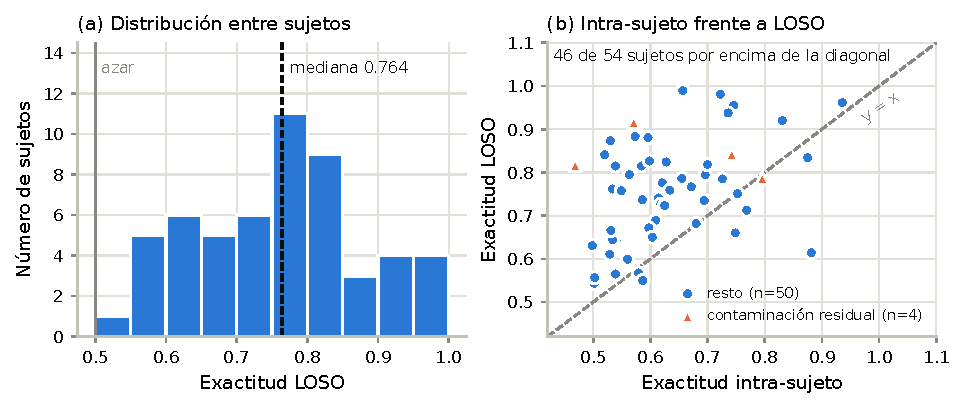
\includegraphics[width=\textwidth]{resultados_baseline.pdf}
\caption{Desempeño de \eegnet{} sobre los 54 sujetos (media de tres semillas). (a) Distribución de la
exactitud \loso{}; la línea continua marca el azar y la discontinua la mediana. (b) Exactitud
intra-sujeto frente a \loso{}; los puntos por encima de la diagonal son sujetos mejor decodificados
con un modelo entrenado en \emph{otras} personas. En naranja, los cuatro sujetos con contaminación
residual. La exactitud intra-sujeto depende del procedimiento de selección del modelo
(subsección~\ref{sec:seleccion-intra}).}
\label{fig:resultados-baseline}
\end{figure}


\subsection{Contraste entre protocolos}
\label{sec:within-vs-loso}

El protocolo \loso{} supera al intra-sujeto de forma sistemática en las cuatro arquitecturas, con
diferencias de $+0.092$ a $+0.145$ y mejoras en $44$ a $51$ de los $54$ sujetos
(tabla~\ref{tab:within-loso}).

\begin{table}[H]
\centering
\caption{Contraste entre validación intra-sujeto y \loso{}, pareado por participante, con la media
de las tres semillas de cada participante en los dos protocolos. El intervalo es de percentiles del
remuestreo de participantes.}
\label{tab:within-loso}
\small
\resizebox{\textwidth}{!}{%
\begin{tabular}{lcccc}
\toprule
 & \textbf{\eegnet{}} & \textbf{Conformer} & \textbf{LaBraM} & \textbf{EEGMamba} \\
\midrule
Exactitud intra-sujeto & 0.634 & 0.602 & 0.663 & 0.571 \\
Exactitud \loso{} & 0.761 & 0.747 & 0.755 & 0.715 \\
\midrule
Diferencia & $+0.126$ & $+0.144$ & $+0.092$ & $+0.145$ \\
IC $95$\,\% & $[+0.092,\ +0.159]$ & $[+0.106,\ +0.180]$ & $[+0.061,\ +0.120]$ & $[+0.117,\ +0.170]$ \\
Sujetos que mejoran con \loso{} & 46 / 54 & 48 / 54 & 44 / 54 & 51 / 54 \\
Wilcoxon pareado & $<0.001$ & $<0.001$ & $<0.001$ & $<0.001$ \\
$r$ & 0.75 & 0.73 & 0.66 & 0.81 \\
\bottomrule
\end{tabular}}
\end{table}

La inversión respecto del patrón habitual de la literatura, en el que el desempeño inter-sujeto cae
por debajo del intra-sujeto \cite{zhu2025hafusenet,li2026survey,brookshire2024}, es compatible con
que la comparación entre protocolos mezcle el cambio de dominio con el volumen de datos de
entrenamiento (unos 18\,000 ensayos frente a 144) y con el procedimiento de evaluación: el
intra-sujeto determina la parada temprana sobre 36 ensayos y evalúa sobre 20, frente a 800 y 400
en \loso{} (subsección~\ref{sec:seleccion-intra}). Con \eegnet{}, la ecuación~\eqref{eq:dsi-clasico} da
una degradación \emph{negativa}:

\begin{equation*}
\mathrm{DSI}_{\text{clásico}} = \frac{0.6343 - 0.7606}{0.6343} = -0.199
\end{equation*}

Los valores de las cuatro arquitecturas ($-0.20$, $-0.24$, $-0.14$ y $-0.25$ con las medias de la
tabla~\ref{tab:conformer}) no siguen el tamaño de los modelos y dependen del procedimiento de selección
del modelo, de modo que el indicador clásico no sirve para ordenarlas ni como medida de robustez.


\subsection{Indicador propuesto}
\label{sec:dsi-resultados}

El indicador \dsi{} de la ecuación~\eqref{eq:dsi} es positivo en las cuatro arquitecturas, entre
$+0.026$ y $+0.052$ (entre el $2.6$ y el $5.2$\,\% en términos relativos), y solo en LaBraM
alcanza significación tras la corrección de Holm ($p_{\text{Holm}} = 0.033$, tabla~\ref{tab:dsi}).
Las columnas de vistos y no vistos proceden de un mismo conjunto de pesos por \textit{fold}, por lo
que la diferencia queda libre del confundidor de volumen de datos de la
ecuación~\eqref{eq:dsi-clasico}.

\begin{table}[H]
\centering
\caption{Indicador \dsi{} de las cuatro arquitecturas sobre los $54$ \textit{folds}
\loso{}. Panel superior: media de las tres semillas por \textit{fold}; panel inferior: semilla
2026 sola. La columna $p$ corresponde al contraste de Wilcoxon
pareado entre participantes vistos y no vistos; $p_{\text{Holm}}$ es su valor corregido por los
cuatro contrastes de cada panel, y $r$ el tamaño de efecto del mismo contraste. En negrita, la
única arquitectura para la que se declara degradación.}
\label{tab:dsi}
\small
\setlength{\tabcolsep}{4pt}
\begin{tabular}{lccccccc}
\toprule
 & \multicolumn{2}{c}{\textbf{Exactitud}} & & & & & \\
\cmidrule(lr){2-3}
 & Vistos & No vistos & \dsi{} & \dsi{} kappa & \textit{Folds} $>0$ & $p$ \;/\; $p_{\text{Holm}}$ & $r$ \\
\midrule
\multicolumn{8}{l}{\textit{Media de tres semillas por \textit{fold} (2026, 2027 y 2028)}} \\
\eegnet{} & 0.781 & 0.761 & $+0.026$ & $+0.071$ & 30/54 & 0.25 \;/\; 0.25 & 0.16 \\
Conformer & 0.775 & 0.747 & $+0.037$ & $+0.103$ & 34/54 & 0.099 \;/\; 0.20 & 0.22 \\
\textbf{LaBraM} & \textbf{0.796} & \textbf{0.755} & \textbf{$+0.052$} & \textbf{$+0.140$} & \textbf{37/54} & \textbf{0.008 \;/\; 0.033} & \textbf{0.36} \\
EEGMamba & 0.742 & 0.715 & $+0.036$ & $+0.110$ & 37/54 & 0.027 \;/\; 0.082 & 0.30 \\
\midrule
\multicolumn{8}{l}{\textit{Semilla 2026 sola}} \\
\eegnet{} & 0.783 & 0.763 & $+0.026$ & $+0.071$ & 33/54 & 0.23 \;/\; 0.23 & 0.16 \\
Conformer & 0.786 & 0.752 & $+0.044$ & $+0.121$ & 34/54 & 0.053 \;/\; 0.11 & 0.26 \\
\textbf{LaBraM} & \textbf{0.798} & \textbf{0.754} & \textbf{$+0.055$} & \textbf{$+0.148$} & \textbf{38/54} & \textbf{0.006 \;/\; 0.026} & \textbf{0.37} \\
EEGMamba & 0.742 & 0.717 & $+0.034$ & $+0.105$ & 37/54 & 0.038 \;/\; 0.11 & 0.28 \\
\bottomrule
\end{tabular}
\end{table}

Sin la corrección de Holm, que se fijó tras conocer los valores de la semilla 2026
(sección~\ref{sec:estadistica}), también EEGMamba ($p = 0.027$) cumpliría el criterio. La magnitud
del indicador es muy inferior a la degradación que el
sección~\ref{cap:validacion-externa} atribuye al cambio de protocolo de adquisición. Sus
intervalos se solapan (subsección~\ref{sec:bootstrap-resultados}), de modo que de estos valores no se
extrae una relación con el número de parámetros, el preentrenamiento o el mecanismo de procesamiento;
los datos tampoco permiten descartar diferencias de tamaño moderado, porque las cuatro arquitecturas
difieren a la vez en esos factores. LaBraM, el único modelo preentrenado, presenta el indicador más
alto. La declaración para LaBraM se sostiene con la semilla 2026 y con la media de tres semillas, y no
con cada una de las otras dos por separado ($p_{\text{Holm}} = 0.074$ y $0.052$). Este resultado es
el primer eje del criterio de la sección~\ref{sec:criterio-robustez} y se retoma en la
sección~\ref{sec:aplicacion-robustez}.

\subsubsection{Restricción de interpretación}

El indicador \textbf{solo admite interpretación agregada}, y no se reporta por sujeto. En kappa, con
\eegnet{} y la media de tres semillas, el conjunto de sujetos vistos promedia $51$ personas y es casi
constante entre \textit{folds} (desviación $0.029$), mientras que el no visto es un solo sujeto
(desviación $0.237$); el \dsi{} de un \textit{fold} es casi una transformación lineal del desempeño
del sujeto de prueba ($r = -0.993$), una consecuencia aritmética de la construcción y no un hallazgo.
Se considera sujeto de bajo rendimiento (\textit{BCI illiteracy}) al que no supera el $70$\,\% de
exactitud \cite{kubler2004,vidaurre2010}; el fenómeno afecta al $15$ a $30$\,\% de los usuarios
\cite{vidaurre2010,blankertz2010} y a una tasa del $53.7$\,\% en \openbmi{} con CSP
\cite{lee2019}. La dificultad del sujeto se trata como un problema de separabilidad de la señal y
no de ausencia de ella \cite{huang2023discrepancy}.


\subsection{Análisis de sensibilidad a los artefactos residuales}
\label{sec:sensibilidad}

Los cuatro sujetos con contaminación ocular residual no determinan la conclusión principal: sin
ellos, el \dsi{} en kappa del resto asciende a $+0.093$ (tabla~\ref{tab:sensibilidad}).

\begin{table}[H]
\centering
\caption{Sujetos con contaminación residual frente al resto (\eegnet{}, \loso{}, media de tres semillas por \textit{fold}).}
\label{tab:sensibilidad}
\begin{tabular}{lccc}
\toprule
 & \textbf{$n$} & \textbf{Exactitud \loso{}} & \textbf{\dsi{} kappa} \\
\midrule
Residuales & 4  & 0.841 & $-0.190$ \\
Resto      & 50 & 0.754 & $+0.093$ \\
\bottomrule
\end{tabular}
\end{table}

Los sujetos marcados por el control ocular tras la limpieza (\texttt{sub-06}, \texttt{sub-29},
\texttt{sub-32} y \texttt{sub-37}) presentan mayor exactitud y \dsi{} negativo, en la dirección que
predice la hipótesis de que la señal ocular residual los vuelve artificialmente fáciles de clasificar.
Con solo cuatro sujetos la diferencia no es concluyente y se reporta como control.


\subsection{Distribución entre sujetos}

La exactitud \loso{} de \eegnet{} varía de $0.543$ a $0.989$ entre sujetos, con $20$ por encima de
$0.80$ y $6$ por debajo de $0.60$ (tabla~\ref{tab:distribucion}).

\begin{table}[H]
\centering
\caption{Distribución de la exactitud \loso{} de \eegnet{} entre los 54 sujetos, con la media de tres semillas por sujeto (igual que la correlación).}
\label{tab:distribucion}
\begin{tabular}{p{7.5cm}c}
\toprule
Cuartiles (Q1 / mediana / Q3) & 0.667 / 0.764 / 0.832 \\
Rango & entre 0.543 (sub-24) y 0.989 (sub-33) \\
Sujetos con exactitud $< 0.60$ & 6 \\
Sujetos con exactitud $> 0.80$ & 20 \\
Correlación de Pearson intra-sujeto frente a \loso{} & 0.36 \\
\bottomrule
\end{tabular}
\end{table}

Los dos protocolos ordenan a los participantes solo en parte: la correlación entre ellos es de
$0.36$ en \eegnet{} y varía de $0.31$ a $0.68$ entre arquitecturas, con el valor más alto en LaBraM y
un intervalo al $95$\,\% del Conformer que incluye el cero ($-0.03$ a $0.59$). Es compatible con que la
facilidad de decodificación dependa del régimen de entrenamiento y con el ruido del protocolo
intra-sujeto (subsección~\ref{sec:seleccion-intra}); los datos no permiten atribuirla a la persona.


\subsection{Comparación entre arquitecturas}
\label{sec:comparacion}

En \loso{}, \eegnet{}, el Conformer y LaBraM \cite{jiang2024labram} (variante Base, con ajuste fino
completo; sección~\ref{sec:representaciones}) no muestran diferencias significativas entre sí y son
equivalentes dentro de $\pm 0.03$, mientras que EEGMamba queda por debajo de las tres con tamaño de
efecto grande. En el protocolo intra-sujeto ninguna comparación es equivalente y las diferencias
dependen del procedimiento de selección del modelo. La tabla~\ref{tab:conformer} contrasta las
cuatro arquitecturas, entrenadas con el esquema unificado y evaluadas sobre las mismas $54$
particiones.

\begin{table}[H]
\centering
\caption{\eegnet{}, Conformer, LaBraM (variante Base) y EEGMamba sobre las mismas 54
particiones, pareado por sujeto, con la media de tres semillas por sujeto. El \dsi{} se calcula como
$(m_{\text{visto}} - m_{\text{no visto}})/m_{\text{visto}}$ sobre las medias
agregadas de los 54 sujetos. El símbolo
$\pm$ es la desviación típica entre los 54 sujetos; para los sujetos vistos es la
desviación entre los 54 \textit{folds}, cada uno con unos 51 participantes, de modo
que no mide dispersión entre personas. El kappa de los sujetos vistos es $2\,\mathrm{exactitud} - 1$.
El valor intra-sujeto de EEGMamba emplea la cabeza que conserva la representación por
canal (sección~\ref{sec:eegmamba-adapt}).}
\label{tab:conformer}
\footnotesize
\setlength{\tabcolsep}{3pt}
\begin{tabular}{lcccc}
\toprule
 & \textbf{\eegnet{}} & \textbf{Conformer} & \textbf{LaBraM} & \textbf{EEGMamba} \\
\midrule
Exactitud intra-sujeto & $0.634 \pm 0.107$ & $0.602 \pm 0.117$ & $0.663 \pm 0.153$ & $0.571 \pm 0.095$ \\
\midrule
Exactitud \loso{}, sujetos vistos & $0.781 \pm 0.014$ & $0.775 \pm 0.032$ & $0.796 \pm 0.010$ & $0.742 \pm 0.009$ \\
Exactitud \loso{}, sujeto no visto & $0.761 \pm 0.119$ & $0.747 \pm 0.121$ & $0.755 \pm 0.107$ & $0.715 \pm 0.103$ \\
\dsi{} (exactitud) & $+0.026$ & $+0.037$ & $+0.052$ & $+0.036$ \\
\midrule
Kappa \loso{}, sujetos vistos & $0.561 \pm 0.029$ & $0.550 \pm 0.064$ & $0.593 \pm 0.020$ & $0.484 \pm 0.019$ \\
Kappa \loso{}, sujeto no visto & $0.521 \pm 0.237$ & $0.494 \pm 0.242$ & $0.510 \pm 0.214$ & $0.431 \pm 0.207$ \\
\dsi{} (kappa) & $+0.071$ & $+0.103$ & $+0.140$ & $+0.110$ \\
\bottomrule
\end{tabular}
\end{table}

Bajo \loso{}, \eegnet{}, el Conformer y LaBraM \textbf{no muestran diferencias
significativas} entre sí (tamaños de efecto $r$ de $0.11$ a $0.24$, tabla~\ref{tab:wilcoxon}) y son
equivalentes dentro de $\pm 0.03$ (subsección~\ref{sec:wilcoxon}). LaBraM presenta el \dsi{} más alto
(\dsi{} kappa $+0.140$), sin que la diferencia sea concluyente. EEGMamba, la única arquitectura de espacio
de estados, alcanza $0.715$ sobre el sujeto no visto y se separa de las otras tres de forma significativa
y con tamaño de efecto grande, con un \dsi{} del orden del de las demás ($+0.036$).

En el protocolo intra-sujeto, \eegnet{} y LaBraM superan al Conformer de forma significativa
(\eegnet{}: $p < 0.001$, $r = 0.59$; LaBraM: $p = 0.001$, $r = 0.44$), y entre ellas no se detecta
diferencia ($p = 0.44$, $r = 0.11$) pero tampoco puede declararse equivalencia, porque la diferencia de
medias ($+0.03$ a favor de LaBraM, intervalo al $90$\,\% de $[+0.001,\ +0.059]$) sale del margen y la mediana
favorece a \eegnet{}. EEGMamba alcanza $0.571$, la cifra más baja pero por encima del azar
($p = 1.2\times10^{-9}$). Estas diferencias no deben leerse como una comparación de capacidad ni de
preentrenamiento: el criterio de parada conserva un modelo de las épocas de calentamiento en entre el
$53.1$ y el $60.3$\,\% de las ejecuciones del Conformer, frente a entre el $12.4$ y el $16.8$\,\% de
\eegnet{} y entre el $21.1$ y el $28.1$\,\% de LaBraM (subsección~\ref{sec:seleccion-intra}).

\subsubsection{Contrastes pareados y tamaño de efecto}
\label{sec:wilcoxon}

En \loso{}, solo EEGMamba se separa de las demás, con $r$ de $0.54$ a $0.74$; en el protocolo
intra-sujeto se separan el Conformer y EEGMamba. La tabla~\ref{tab:wilcoxon} recoge las seis
comparaciones por protocolo (Wilcoxon pareado, $n = 54$) con el tamaño de efecto
$r = |Z|/\sqrt{n}$ (referencia habitual: $0.1$ pequeño, $0.3$ mediano, $0.5$ grande).

\begin{table}[H]
\centering
\caption{Contrastes de Wilcoxon pareados sobre los 54 participantes, con la media de las tres
semillas de cada participante, y tamaño de efecto $r = |Z|/\sqrt{n}$. La diferencia
mediana corresponde a la primera arquitectura menos la segunda. Cada protocolo y cada métrica
forman una familia de seis contrastes; con la corrección de Holm (exactitud) ninguna conclusión de
significación cambia. Los valores $p$ son bilaterales. En negrita, $r \geq 0.5$. Los resultados por
semilla figuran en la tabla~\ref{tab:variabilidad-dif}.}
\label{tab:wilcoxon}
\small
\begin{tabular}{lrrrrrrr}
\toprule
& \multicolumn{4}{c}{\textbf{Exactitud}} & \multicolumn{3}{c}{\textbf{Kappa}} \\
\cmidrule(lr){2-5}\cmidrule(lr){6-8}
\textbf{Comparación} & \textbf{dif.} & $p$ & $p_{\text{Holm}}$ & $r$ & \textbf{dif.} & $p$ & $r$ \\
\midrule
\multicolumn{8}{l}{\textit{Inter-sujeto (\loso{})}} \\
\eegnet{} vs Conformer & $+0.006$ & 0.073 & 0.22 & $0.24$ & $+0.013$ & 0.073 & $0.24$ \\
\eegnet{} vs LaBraM & $+0.002$ & 0.42 & 0.42 & $0.11$ & $+0.004$ & 0.42 & $0.11$ \\
Conformer vs LaBraM & $-0.008$ & 0.19 & 0.38 & $0.18$ & $-0.017$ & 0.19 & $0.18$ \\
\eegnet{} vs EEGMamba & $+0.045$ & $<0.001$ & $<0.001$ & $\mathbf{0.73}$ & $+0.091$ & $<0.001$ & $\mathbf{0.73}$ \\
Conformer vs EEGMamba & $+0.036$ & $<0.001$ & $<0.001$ & $\mathbf{0.54}$ & $+0.072$ & $<0.001$ & $\mathbf{0.54}$ \\
LaBraM vs EEGMamba & $+0.039$ & $<0.001$ & $<0.001$ & $\mathbf{0.74}$ & $+0.078$ & $<0.001$ & $\mathbf{0.74}$ \\
\midrule
\multicolumn{8}{l}{\textit{Intra-sujeto}} \\
\eegnet{} vs Conformer & $+0.033$ & $<0.001$ & $<0.001$ & $\mathbf{0.59}$ & $+0.067$ & $<0.001$ & $\mathbf{0.59}$ \\
\eegnet{} vs LaBraM & $+0.018$ & 0.44 & 0.44 & $0.11$ & $+0.037$ & 0.44 & $0.11$ \\
Conformer vs LaBraM & $-0.034$ & 0.001 & 0.002 & $0.44$ & $-0.068$ & 0.001 & $0.44$ \\
\eegnet{} vs EEGMamba & $+0.064$ & $<0.001$ & $<0.001$ & $\mathbf{0.73}$ & $+0.127$ & $<0.001$ & $\mathbf{0.73}$ \\
Conformer vs EEGMamba & $+0.027$ & $<0.001$ & $<0.001$ & $\mathbf{0.54}$ & $+0.053$ & $<0.001$ & $\mathbf{0.54}$ \\
LaBraM vs EEGMamba & $+0.044$ & $<0.001$ & $<0.001$ & $\mathbf{0.80}$ & $+0.088$ & $<0.001$ & $\mathbf{0.80}$ \\
\bottomrule
\end{tabular}
\end{table}

\eegnet{}, el Conformer y LaBraM son \textbf{equivalentes dentro del margen de $\pm 0.03$} en
\loso{} (tabla~\ref{tab:equivalencia}): con la media de tres semillas, los intervalos al $90$\,\% de
sus diferencias son $[+0.004,\ +0.025]$ (\eegnet{} y Conformer), $[-0.003,\ +0.015]$ (\eegnet{} y
LaBraM) y $[-0.018,\ +0.002]$ (Conformer y LaBraM), de modo que la equivalencia valdría para cualquier
margen superior a $0.025$. Tres salvedades la acotan: el margen se fijó tras un primer análisis de los
datos y es del orden de la diferencia entre vistos y no vistos ($0.02$ a $0.04$), por lo que no excluye
diferencias de la magnitud del efecto que estudia el \dsi{}; las semillas no comparten régimen de
optimización, aunque la equivalencia se mantiene con las semillas $2027$ y $2028$ solas
(subsección~\ref{sec:confusor}); y la dispersión entre semillas de las diferencias, de $0.001$ a $0.006$,
se estima con tres valores (subsección~\ref{sec:variabilidad-semillas}).

EEGMamba no resultó equivalente a ninguna de las otras tres: sus intervalos al $90$\,\% son
$[+0.035,\ +0.056]$ frente a \eegnet{} y $[+0.018,\ +0.044]$ frente al Conformer.

Frente a LaBraM, el intervalo fue $[+0.030,\ +0.048]$. La separación se mantuvo con las semillas $2027$ y $2028$ solas.

En el protocolo intra-sujeto el Conformer difirió de \eegnet{} y de LaBraM con efectos grande y mediano
($r = 0.59$ y $0.44$) y ningún contraste cumplió la equivalencia, con la salvedad de la
subsección~\ref{sec:seleccion-intra}. EEGMamba se incluyó en esos contrastes con la cabeza \texttt{flatten},
con la que alcanzó $0.571$, frente a una exactitud próxima al azar con la cabeza de promediado global
($0.519$, semilla 2026); queda por debajo de las otras tres y es la más afectada por la selección del
modelo.

\paragraph{Selección del modelo en el protocolo intra-sujeto}
\label{sec:seleccion-intra}

Con $36$ ensayos de validación, frente a los $800$ de \loso{}, el criterio de parada del protocolo
intra-sujeto conserva con frecuencia un modelo de las diez épocas de calentamiento (parada en la
época $30$, el mínimo del esquema): en el Conformer en más de la mitad de las ejecuciones y en
EEGMamba en casi todas (tabla~\ref{tab:seleccion-intra}).

\begin{table}[H]
\centering
\caption{Proporción de ejecuciones en que el modelo conservado procede de las diez épocas de
calentamiento, por semilla y protocolo. Cada proporción es sobre 54 ejecuciones en \loso{} y
sobre 1\,080 en el protocolo intra-sujeto.}
\label{tab:seleccion-intra}
\small
\begin{tabular}{lcccccc}
\toprule
 & \multicolumn{3}{c}{\textbf{Intra-sujeto}} & \multicolumn{3}{c}{\textbf{\loso{}}} \\
\cmidrule(lr){2-4}\cmidrule(lr){5-7}
 & 2026 & 2027 & 2028 & 2026 & 2027 & 2028 \\
\midrule
\eegnet{} & 16.6\,\% & 16.8\,\% & 12.4\,\% & 7.4\,\% & 7.4\,\% & 3.7\,\% \\
Conformer & 53.1\,\% & 59.3\,\% & 60.3\,\% & 13.0\,\% & 25.9\,\% & 18.5\,\% \\
LaBraM & 21.1\,\% & 28.1\,\% & 24.8\,\% & 25.9\,\% & 33.3\,\% & 24.1\,\% \\
EEGMamba & 85.6\,\% & 88.6\,\% & 86.3\,\% & 46.3\,\% & 46.3\,\% & 40.7\,\% \\
\bottomrule
\end{tabular}
\end{table}

\begin{table}[H]
\centering
\caption{Exactitud media de las ejecuciones cuyo modelo conservado procede de las diez épocas de
calentamiento (Esas, con su número entre paréntesis) y de las demás (Resto), con las tres semillas
agrupadas: $3\,240$ ejecuciones por arquitectura en intra-sujeto y $162$ en \loso{}. La unidad es la
ejecución y no el participante; la comparación es descriptiva.}
\label{tab:seleccion-exactitud}
\small
\begin{tabular}{lcccc}
\toprule
 & \multicolumn{2}{c}{\textbf{Intra-sujeto}} & \multicolumn{2}{c}{\textbf{\loso{}}} \\
\cmidrule(lr){2-3}\cmidrule(lr){4-5}
 & Esas & Resto & Esas & Resto \\
\midrule
\eegnet{}  & 0.511 (494)  & 0.656 & 0.724 (10) & 0.763 \\
Conformer  & 0.521 (1865) & 0.714 & 0.685 (31) & 0.761 \\
LaBraM     & 0.521 (800)  & 0.710 & 0.707 (45) & 0.773 \\
EEGMamba   & 0.541 (2814) & 0.767 & 0.703 (72) & 0.725 \\
\bottomrule
\end{tabular}
\end{table}

En esas ejecuciones la exactitud media intra-sujeto es de $0.51$ a $0.54$, próxima al azar, frente a
$0.66$ a $0.77$ en las restantes (tabla~\ref{tab:seleccion-exactitud}); la comparación es descriptiva,
porque las ejecuciones que prolongan el entrenamiento pueden corresponder a participantes más
favorables. Por tanto, la exactitud intra-sujeto del Conformer y de EEGMamba refleja en buena parte el
comportamiento del criterio de selección con $36$ ensayos y no solo la capacidad de aprender de $144$,
y las diferencias intra-sujeto entre arquitecturas no pueden atribuirse a la capacidad ni al
preentrenamiento. En \loso{} el fenómeno es menos frecuente (la mayor proporción es la de EEGMamba,
de $40.7$ a $46.3$\,\%) y la exactitud de las ejecuciones afectadas difiere poco de la del resto
($0.703$ frente a $0.725$).

\paragraph{Número de semillas por arquitectura}
\label{sec:semillas-por-arq}

Las cuatro arquitecturas se ejecutaron con tres semillas ($2026$, $2027$ y $2028$) en los protocolos
intra-sujeto, \loso{} y de transferencia, lo que da $54 \times 20 \times 3 = 3\,240$ mediciones
intra-sujeto y $54 \times 3 = 162$ \textit{folds} \loso{} por arquitectura
(sección~\ref{sec:semillas-metodo}). El régimen de optimización no es el mismo en todas: \eegnet{}, el
Conformer y LaBraM tienen la semilla $2026$ sin recorte de gradiente y las otras dos con él, salvo en el
protocolo intra-sujeto de \eegnet{} y del Conformer, donde las tres se entrenaron sin recorte
(tabla~\ref{tab:regimen}); la subsección~\ref{sec:confusor} acota cuánto puede haber contribuido ese cambio.

La mayor dispersión intra-sujeto de LaBraM ($0.153$ frente a $0.107$ de \eegnet{}) procede de la
variabilidad entre participantes y no de las semillas: la desviación entre semillas de la exactitud media
es de $0.001$ a $0.006$, y la de un mismo participante de $0.016$ a $0.025$, frente a $0.095$ a $0.153$
entre participantes. Los contrastes pareados emplean la media de las tres semillas de cada participante
(sección~\ref{sec:estadistica}).

\subsubsection{Intervalos de confianza por remuestreo}
\label{sec:bootstrap-resultados}

Los intervalos por remuestreo (sección~\ref{sec:bootstrap}, tabla~\ref{tab:bootstrap}) confirman las
conclusiones anteriores: el \dsi{} excluye el cero solo en LaBraM, y la separación de EEGMamba es el
único ordenamiento entre arquitecturas que el remuestreo sostiene.

\begin{table}[htbp]
\centering
\caption{Intervalos de confianza al $95$\,\% por remuestreo jerárquico con reemplazo (participantes
y, dentro de cada participante, sus tres semillas), $B = 10\,000$, semilla $2026$, sobre los $54$
valores por participante, para el \dsi{} y las diferencias entre arquitecturas con la media de tres
semillas. En las diferencias, la extracción de participantes es común a las dos arquitecturas del
par. El intervalo es de percentiles (2.5 y 97.5) de las $B$ réplicas. Las filas de exactitud
(bloque inferior) son la media de tres semillas, con el mismo remuestreo jerárquico.}
\label{tab:bootstrap}
\small
\begin{tabular}{lccc}
\toprule
 & \textbf{Estimación} & \textbf{IC $95$\,\%} & \textbf{Amplitud} \\
\midrule
\multicolumn{4}{l}{\textit{\dsi{}, media de tres semillas}} \\
\eegnet{} & $+0.026$ & $[-0.016,\ +0.068]$ & 0.084 \\
Conformer & $+0.037$ & $[-0.005,\ +0.078]$ & 0.084 \\
LaBraM & $+0.052$ & $[+0.016,\ +0.088]$ & 0.072 \\
EEGMamba & $+0.036$ & $[-0.002,\ +0.074]$ & 0.076 \\
\midrule
\multicolumn{4}{l}{\textit{Diferencia de exactitud \loso{}, media pareada de tres semillas}} \\
\eegnet{} $-$ Conformer & $+0.014$ & $[+0.000,\ +0.029]$ & 0.029 \\
\eegnet{} $-$ LaBraM & $+0.006$ & $[-0.006,\ +0.018]$ & 0.023 \\
Conformer $-$ LaBraM & $-0.008$ & $[-0.022,\ +0.006]$ & 0.028 \\
\eegnet{} $-$ EEGMamba & $+0.045$ & $[+0.032,\ +0.058]$ & 0.026 \\
Conformer $-$ EEGMamba & $+0.032$ & $[+0.014,\ +0.048]$ & 0.034 \\
LaBraM $-$ EEGMamba & $+0.040$ & $[+0.028,\ +0.050]$ & 0.023 \\
\midrule
\multicolumn{4}{l}{\textit{Diferencia de exactitud intra-sujeto, media pareada de tres semillas}} \\
\eegnet{} $-$ Conformer & $+0.032$ & $[+0.018,\ +0.045]$ & 0.027 \\
\eegnet{} $-$ LaBraM & $-0.029$ & $[-0.065,\ +0.005]$ & 0.070 \\
Conformer $-$ LaBraM & $-0.061$ & $[-0.093,\ -0.031]$ & 0.062 \\
\eegnet{} $-$ EEGMamba & $+0.063$ & $[+0.046,\ +0.082]$ & 0.036 \\
Conformer $-$ EEGMamba & $+0.032$ & $[+0.018,\ +0.047]$ & 0.029 \\
LaBraM $-$ EEGMamba & $+0.093$ & $[+0.063,\ +0.123]$ & 0.060 \\
\bottomrule
\end{tabular}

\medskip
\small
\begin{tabular}{lccc}
\toprule
 & \textbf{Estimación} & \textbf{IC $95$\,\%} & \textbf{Amplitud} \\
\midrule
\multicolumn{4}{l}{\textit{Media de tres semillas, remuestreo jerárquico}} \\
\multicolumn{4}{l}{\textit{Exactitud \loso{}}} \\
\eegnet{}  & 0.761 & $[0.728,\ 0.792]$ & 0.064 \\
Conformer  & 0.747 & $[0.714,\ 0.780]$ & 0.066 \\
LaBraM     & 0.755 & $[0.726,\ 0.783]$ & 0.057 \\
EEGMamba   & 0.715 & $[0.688,\ 0.743]$ & 0.055 \\
\midrule
\multicolumn{4}{l}{\textit{Exactitud intra-sujeto}} \\
\eegnet{}  & 0.634 & $[0.606,\ 0.664]$ & 0.058 \\
Conformer  & 0.602 & $[0.572,\ 0.635]$ & 0.062 \\
LaBraM     & 0.663 & $[0.624,\ 0.706]$ & 0.082 \\
EEGMamba   & 0.571 & $[0.547,\ 0.598]$ & 0.050 \\
\bottomrule
\end{tabular}
\end{table}

Las diferencias entre \eegnet{}, el Conformer y LaBraM en \loso{} tienen intervalos de amplitud
$0.023$ a $0.029$ que contienen el cero, salvo el de \eegnet{} frente al Conformer, que lo excluye por
$0.0005$ sin corregir por las seis comparaciones y con $p = 0.073$ en el contraste pareado; no se
declara diferencia. Los intervalos de las tres diferencias que involucran a EEGMamba
($[+0.032,\ +0.058]$, $[+0.014,\ +0.048]$ y $[+0.028,\ +0.050]$) excluyen el cero con holgura. La tabla
reporta diferencias \emph{medias}, y la tabla~\ref{tab:wilcoxon} diferencias \emph{medianas}; pueden
discrepar (entre \eegnet{} y el Conformer, $+0.006$ y $+0.014$) por la asimetría de la distribución por
participante. Al parear por participante la variabilidad entre personas se cancela en buena parte y la
inicialización pasa a ser del $17$ al $35$\,\% de la varianza de la diferencia en \loso{}
(subsección~\ref{sec:variabilidad-semillas}).

\subsubsection{Variabilidad por semilla de las diferencias pareadas}
\label{sec:variabilidad-semillas}

La diferencia media entre arquitecturas tiene el mismo signo en las tres semillas en los $12$
contrastes de exactitud, y ninguna conclusión de significación ni de equivalencia cambia con tres
semillas (tabla~\ref{tab:variabilidad-dif}). Lo que varía entre semillas es el valor $p$ de una semilla
sola y, en los contrastes pequeños de \loso{}, la propia diferencia.

\begin{table}[H]
\centering
\caption{Diferencia media de exactitud (primera menos segunda arquitectura) en cada semilla, desviación
típica (DT) entre las tres semillas de esa diferencia, valores $p$ de Wilcoxon de cada semilla por separado
(2026 / 2027 / 2028) e intervalo al $95$\,\% jerárquico de la diferencia de la media de tres
semillas.}
\label{tab:variabilidad-dif}
\footnotesize
\setlength{\tabcolsep}{3pt}
\resizebox{\textwidth}{!}{%
\begin{tabular}{lccccll}
\toprule
 & \multicolumn{3}{c}{\textbf{Dif. media por semilla}} & & & \\
\cmidrule(lr){2-4}
\textbf{Contraste} & 2026 & 2027 & 2028 & DT & $p$ por semilla & IC $95$\,\% (media de 3) \\
\midrule
\multicolumn{7}{l}{\textit{Inter-sujeto (\loso{})}} \\
\eegnet{} $-$ Conformer & $+0.011$ & $+0.015$ & $+0.015$ & 0.0025 & 0.12 / 0.063 / 0.49 & $[+0.000,\ +0.029]$ \\
\eegnet{} $-$ LaBraM & $+0.009$ & $+0.006$ & $+0.002$ & 0.0035 & 0.27 / 0.41 / 0.88 & $[-0.006,\ +0.018]$ \\
Conformer $-$ LaBraM & $-0.002$ & $-0.009$ & $-0.013$ & 0.0055 & 0.49 / 0.32 / 0.50 & $[-0.022,\ +0.006]$ \\
\eegnet{} $-$ EEGMamba & $+0.046$ & $+0.046$ & $+0.044$ & 0.0008 & $<0.001$ / $<0.001$ / $<0.001$ & $[+0.032,\ +0.058]$ \\
Conformer $-$ EEGMamba & $+0.035$ & $+0.030$ & $+0.029$ & 0.0030 & $<0.001$ / $<0.001$ / $<0.001$ & $[+0.014,\ +0.048]$ \\
LaBraM $-$ EEGMamba & $+0.037$ & $+0.039$ & $+0.042$ & 0.0027 & $<0.001$ / $<0.001$ / $<0.001$ & $[+0.028,\ +0.050]$ \\
\midrule
\multicolumn{7}{l}{\textit{Intra-sujeto}} \\
\eegnet{} $-$ Conformer & $+0.026$ & $+0.031$ & $+0.038$ & 0.0062 & $<0.001$ / $<0.001$ / $<0.001$ & $[+0.018,\ +0.045]$ \\
\eegnet{} $-$ LaBraM & $-0.032$ & $-0.033$ & $-0.023$ & 0.0052 & 0.30 / 0.31 / 0.58 & $[-0.065,\ +0.005]$ \\
Conformer $-$ LaBraM & $-0.058$ & $-0.063$ & $-0.061$ & 0.0028 & 0.004 / 0.001 / $<0.001$ & $[-0.093,\ -0.031]$ \\
\eegnet{} $-$ EEGMamba & $+0.056$ & $+0.060$ & $+0.074$ & 0.0097 & $<0.001$ / $<0.001$ / $<0.001$ & $[+0.046,\ +0.082]$ \\
Conformer $-$ EEGMamba & $+0.030$ & $+0.029$ & $+0.036$ & 0.0038 & $<0.001$ / $<0.001$ / $<0.001$ & $[+0.018,\ +0.047]$ \\
LaBraM $-$ EEGMamba & $+0.088$ & $+0.092$ & $+0.098$ & 0.0049 & $<0.001$ / $<0.001$ / $<0.001$ & $[+0.063,\ +0.123]$ \\
\bottomrule
\end{tabular}
}
\end{table}

La desviación entre semillas de la diferencia media va de $0.0008$ a $0.0055$ en \loso{} y de $0.003$ a
$0.010$ en el protocolo intra-sujeto. En los contrastes pequeños de \loso{} es del orden del propio
efecto (\eegnet{} frente a LaBraM vale $+0.009$, $+0.006$ y $+0.002$ en las tres semillas) y en los de
EEGMamba es despreciable. El valor $p$ de una semilla sola puede cambiar mucho: \eegnet{} frente al
Conformer en \loso{} da $0.12$, $0.063$ y $0.49$, y $0.073$ con la media de las tres. El ruido de semilla
explica del $17$ al $35$\,\% de la varianza entre participantes de la diferencia media en \loso{} y del
$2$ al $23$\,\% en el protocolo intra-sujeto.

No se detecta que el cambio de régimen modifique estas diferencias. El desplazamiento entre la diferencia
de la semilla $2026$ y la de las semillas $2027$ y $2028$ va de $-0.011$ a $+0.009$ en los doce contrastes,
con intervalos al $95$\,\% que contienen el cero, y en el contraste sin cambio de régimen (\eegnet{}
frente al Conformer en intra-sujeto) vale $-0.008$ $[-0.018,\ +0.001]$. La resolución de esta comparación
es de $\pm 0.01$ a $\pm 0.02$, de modo que los datos no distinguen el efecto del régimen del ruido
entre semillas.

En la transferencia, las semillas cambian la estimación puntual y no la inferencia: la desviación entre
semillas de la diferencia entre la caída por protocolo y por persona es de $0.003$ a $0.029$, frente a
una semianchura del intervalo de $0.12$ a $0.16$. Con tres semillas la desviación entre semillas tiene
dos grados de libertad, el emparejamiento de semillas entre arquitecturas solo las etiqueta por índice y
las semillas no son réplicas del mismo entorno (subsección~\ref{sec:semillas-por-arq}); la variabilidad por
semilla queda estimada solo de forma aproximada.

\subsubsection{Equivalencia práctica en ambos protocolos}
\label{sec:equivalencia-resultados}

En \loso{}, \eegnet{}, el Conformer y LaBraM son equivalentes dentro de $\pm 0.03$ y EEGMamba no es
equivalente a ninguna; en el protocolo intra-sujeto ningún par lo es (tabla~\ref{tab:equivalencia}). Como
el margen se fijó tras un primer análisis de los datos, se informa también el menor margen con el que se
cumpliría la equivalencia.

\begin{table}[H]
\centering
\caption{Equivalencia práctica con margen $\pm 0.03$ en exactitud. Entre paréntesis, si el
intervalo al $90$\,\% queda dentro del margen. Margen mín.: mayor valor absoluto de los extremos
del intervalo con la media de tres semillas. $p_{\text{TOST,Holm}}$: contraste TOST con la prueba
de Wilcoxon, corregido por Holm en la familia de seis.}
\label{tab:equivalencia}
\small
\resizebox{\textwidth}{!}{%
\begin{tabular}{lllcc}
\toprule
\textbf{Contraste} & IC $90$\,\% (2026) & IC $90$\,\% (media de 3) & Margen mín. & $p_{\text{TOST,Holm}}$ \\
\midrule
\multicolumn{5}{l}{\textit{Inter-sujeto (\loso{})}} \\
\eegnet{} $-$ Conformer & $[+0.002,\ +0.020]$ (sí) & $[+0.004,\ +0.025]$ (sí) & 0.025 & 0.001 \\
\eegnet{} $-$ LaBraM & $[-0.002,\ +0.020]$ (sí) & $[-0.003,\ +0.015]$ (sí) & 0.015 & $<0.001$ \\
Conformer $-$ LaBraM & $[-0.013,\ +0.009]$ (sí) & $[-0.018,\ +0.002]$ (sí) & 0.018 & 0.003 \\
\eegnet{} $-$ EEGMamba & $[+0.035,\ +0.057]$ (no) & $[+0.035,\ +0.056]$ (no) & 0.056 & 1.00 \\
Conformer $-$ EEGMamba & $[+0.023,\ +0.046]$ (no) & $[+0.018,\ +0.044]$ (no) & 0.044 & 1.00 \\
LaBraM $-$ EEGMamba & $[+0.028,\ +0.046]$ (no) & $[+0.030,\ +0.048]$ (no) & 0.048 & 1.00 \\
\midrule
\multicolumn{5}{l}{\textit{Intra-sujeto}} \\
\eegnet{} $-$ Conformer & $[+0.014,\ +0.038]$ (no) & $[+0.021,\ +0.042]$ (no) & 0.042 & 1.00 \\
\eegnet{} $-$ LaBraM & $[-0.062,\ -0.002]$ (no) & $[-0.059,\ -0.001]$ (no) & 0.059 & 1.00 \\
Conformer $-$ LaBraM & $[-0.085,\ -0.032]$ (no) & $[-0.087,\ -0.036]$ (no) & 0.087 & 1.00 \\
\eegnet{} $-$ EEGMamba & $[+0.040,\ +0.073]$ (no) & $[+0.049,\ +0.078]$ (no) & 0.078 & 1.00 \\
Conformer $-$ EEGMamba & $[+0.017,\ +0.044]$ (no) & $[+0.020,\ +0.044]$ (no) & 0.044 & 1.00 \\
LaBraM $-$ EEGMamba & $[+0.063,\ +0.113]$ (no) & $[+0.068,\ +0.118]$ (no) & 0.118 & 1.00 \\
\bottomrule
\end{tabular}
}
\end{table}

La equivalencia en \loso{} se mantiene con la media de tres semillas, con el intervalo jerárquico y con las
semillas $2027$ y $2028$ solas (todas con recorte de gradiente). El menor margen es de $0.025$ para
\eegnet{} frente al Conformer con tres semillas y de $0.029$ con las semillas $2027$ y $2028$, de modo que
en ese par la conclusión queda justo dentro del margen y no vale para márgenes menores. El TOST con la
prueba de Wilcoxon la confirma ($p_{\text{Holm}}$ de $0.001$, $<0.001$ y $0.003$), y el TOST con la $t$ de
Student, más conservador, también. Con EEGMamba los márgenes mínimos son de $0.044$ a $0.056$.

En el protocolo intra-sujeto \textbf{ningún contraste es equivalente}: el menor margen va de $0.042$ a
$0.118$ con tres semillas. \eegnet{} frente a LaBraM, sin diferencia detectable ($p = 0.44$), tampoco es
equivalente, de modo que no puede declararse ni diferencia ni igualdad.


\section{Prueba 2: variantes de preprocesamiento, alineamiento y calibración}
\subsection{Descripción}
Se midió la asociación de las variantes de preprocesamiento, aumentación, alineamiento y calibración con la exactitud, frente a sus referencias correspondientes.
\subsection{Procedimiento}
Las variantes se compararon de forma pareada por sujeto, con la semilla 2026 y las familias de contraste de la sección~\ref{sec:estadistica-variantes}; la calibración empleó los procedimientos de la sección~\ref{sec:metodo-fewshot}.
\subsection{Condiciones de lectura de las variantes}
\label{sec:condiciones-variantes}

Todas las variantes se comparan con la base de \textbf{la misma semilla} ($2026$), en contraste pareado
por participante ($n = 54$) y con los estadísticos de la sección~\ref{sec:estadistica-variantes}. Los
contrastes en kappa coinciden con los de exactitud y no se repiten. Las comparaciones múltiples se
corrigen con Holm dentro de las familias declaradas de antemano (tabla~\ref{tab:familias}); lo que no
pertenece a ninguna familia se rotula exploratorio y no se corrige.

\begin{table}[H]
\centering
\caption{Familias de contrastes de las variantes y de las semillas adicionales, declaradas antes de calcular los resultados.
Cada familia se corrige con Holm por separado. Las dos familias secundarias son informativas.}
\label{tab:familias}
\small
\begin{tabular}{p{3.6cm}p{8.6cm}c}
\toprule
\textbf{Familia} & \textbf{Contenido} & $m$ \\
\midrule
Entre arquitecturas & Seis pares por protocolo y métrica, con la media de tres semillas (la misma estructura que con la semilla $2026$ sola) & 6 \\
Ablaciones intra-sujeto, \eegnet{} y Conformer & Ocho variantes frente a la base intra-sujeto de la semilla 2026: tres subbandas, dos ventanas, sin aumentación, reflexión de canales y ruido en Fourier & 8 \\
Ablaciones intra-sujeto recortadas, LaBraM y EEGMamba & Reflexión de canales, ruido en Fourier y ventana de \seg{0} a \seg{2} (recorte decidido antes de ejecutar) & 3 \\
Alineamiento euclidiano en \loso{} & \loso{} con alineamiento euclidiano frente a la base \loso{} de la semilla 2026, uno por arquitectura & 4 \\
Reflexión de canales en \loso{} & \loso{} con reflexión de canales frente a la misma base, uno por arquitectura & 4 \\
Calibración, base y alineamiento & Cuatro arquitecturas, dos tamaños de calibración y tres métodos; la familia de los modelos base y la de los modelos con alineamiento se corrigen por separado & 24 y 24 \\
Políticas de normalización & Origen frente a las otras dos políticas, por arquitectura & 8 \\
Alineamiento en la transferencia & Tres evaluaciones por cuatro arquitecturas, variante con alineamiento frente a la base de la semilla 2026 & 12 \\
\midrule
Secundarias & Los $22$ contrastes de las ablaciones intra-sujeto a la vez, y los $8$ de alineamiento y reflexión en \loso{} a la vez & 22 y 8 \\
\bottomrule
\end{tabular}
\end{table}

\subsubsection{Variantes evaluadas}

Las variantes y su implementación se describen en las secciones~\ref{sec:variantes-banda},
\ref{sec:variantes-aug} y~\ref{sec:variantes-ea}. Para leer los resultados basta saber que la variante
sin aumentación anula las tres transformaciones de la base, que la amplitud $0.1$ del ruido en Fourier es
una elección propia y que el alineamiento es transductivo: el participante de prueba se alinea con sus
propios segmentos sin etiqueta.

\subsubsection{Cota del efecto del recorte de gradiente}
\label{sec:confusor}

Los datos descartan un efecto medio del cambio de régimen (recorte de gradiente, hardware y código)
superior a entre $0.010$ y $0.020$ de exactitud según la arquitectura, no que el efecto sea nulo
(tabla~\ref{tab:confusor}). En \eegnet{}, el Conformer y LaBraM el contraste de una variante con su base
está confundido con ese cambio (tabla~\ref{tab:regimen}); EEGMamba no cambia de recorte, aunque sí de
hardware y de versión del código. El procedimiento de la cota está en la
sección~\ref{sec:cota-confusor}.

\begin{table}[H]
\centering
\caption{Diferencia por participante entre la semilla $2026$ (sin recorte) y la media de las
semillas $2027$ y $2028$ (con recorte), con intervalo al $95$\,\% de percentiles, y cota resultante.
La cota neta resta la misma diferencia en EEGMamba, que no cambia de recorte. Solo existe donde la base cambia
de régimen entre semillas.}
\label{tab:confusor}
\small
\begin{tabular}{llccc}
\toprule
\textbf{Protocolo} & \textbf{Arq.} & Delta bruto, IC $95$\,\% & Cota bruta & Cota neta \\
\midrule
\loso{} & \eegnet{} & $+0.0030$ $[-0.0042,\ +0.0104]$ & 0.0104 & 0.0100 \\
\loso{} & Conformer & $+0.0072$ $[-0.0043,\ +0.0198]$ & 0.0198 & 0.0178 \\
\loso{} & LaBraM & $-0.0016$ $[-0.0097,\ +0.0063]$ & 0.0097 & 0.0142 \\
Intra-sujeto & LaBraM & $+0.0021$ $[-0.0051,\ +0.0092]$ & 0.0092 & 0.0182 \\
\bottomrule
\end{tabular}
\end{table}

Ninguna de las cuatro diferencias medias se distingue de cero (Wilcoxon, $p$ de $0.37$ a $0.91$). En una
media de tres semillas, con una de ellas sin recorte, la contaminación máxima sería la tercera parte, de
$0.003$ a $0.007$. En EEGMamba, que no cambia de recorte, la misma diferencia llega a $+0.009$ en el
protocolo intra-sujeto ($p$ sin corregir de $0.048$), del orden de las cotas, lo que es compatible con
ruido de semilla y con el cambio de hardware y de código. En el protocolo intra-sujeto de \eegnet{} y el
Conformer, que nunca tuvieron recorte, la cota no es estimable. La regla de lectura, fijada de antemano:
un efecto que no supera la cota se declara \emph{no interpretable}, no \emph{sin efecto}; sin cota
estimable, el resultado se informa como condicionado al régimen.


\subsection{Ablaciones intra-sujeto de preprocesamiento y aumentación}
\label{sec:ablaciones-f4}

Ningún efecto de preprocesamiento o aumentación es común a las cuatro arquitecturas: la ventana corta, la
banda $\mu+\beta$ y la reflexión de canales se asocian con una exactitud mayor en algunas y no en otras
(tabla~\ref{tab:ablaciones-f4}). Los resultados de \eegnet{} y el Conformer están \emph{condicionados al
régimen de entrenamiento}, porque no existe una base con recorte con la que estimar una cota
(subsección~\ref{sec:confusor}); en LaBraM la cota es de $0.0182$, y el contraste de EEGMamba no cambia de
recorte, aunque el desplazamiento de $+0.009$ de esa arquitectura entre semillas es del orden de varios
de los efectos de la tabla. Todas las variantes tienen una sola semilla, por lo que las equivalencias valen
para la semilla $2026$ (el desplazamiento medio entre semillas llega a $0.008$ y $0.009$). Los efectos se
describen como asociaciones: no se contrastó la interacción entre arquitectura y variante.

\begin{table}[H]
\centering
\caption{Ablaciones intra-sujeto: diferencia de exactitud de la variante menos la base de la semilla
$2026$, sobre los $54$ participantes, con intervalo al $95$\,\% de percentiles y $p_{\text{Holm}}$ dentro de la
familia de la arquitectura (ocho contrastes en \eegnet{} y Conformer, tres en LaBraM y EEGMamba). Margen
mín.: menor margen con el que se cumpliría la equivalencia (equivalente dentro de $\pm 0.03$ si
es $\leq 0.030$). Lectura: \emph{sin cambio de recorte} (EEGMamba); \emph{sin cota
estimable}, condicionado al régimen (\eegnet{} y Conformer); \emph{supera la cota} o \emph{no
interpretable}, según la magnitud frente a la cota de $0.0182$ (LaBraM).}
\label{tab:ablaciones-f4}
\footnotesize
\setlength{\tabcolsep}{3pt}
\resizebox{\textwidth}{!}{%
\begin{tabular}{llccccl}
\toprule
\textbf{Arq.} & \textbf{Variante} & Dif. media & IC $95$\,\% & $p_{\text{Holm}}$ & Margen mín. & Lectura \\
\midrule
\eegnet{} & banda $\mu$ ($8$ a $13$\,Hz) & $-0.0300$ & $[-0.0635,\ +0.0032]$ & 0.49 & 0.058 & sin cota estimable \\
 & banda $\beta$ ($13$ a $30$\,Hz) & $-0.0456$ & $[-0.0788,\ -0.0098]$ & 0.009 & 0.073 & sin cota estimable \\
 & banda $\mu+\beta$ ($8$ a $30$\,Hz) & $-0.0060$ & $[-0.0450,\ +0.0342]$ & 0.90 & 0.039 & sin cota estimable \\
 & ventana $0$ a $2$\,s & $+0.0417$ & $[+0.0294,\ +0.0541]$ & $<0.001$ & 0.052 & sin cota estimable \\
 & ventana $0$ a $3$\,s & $+0.0045$ & $[-0.0054,\ +0.0145]$ & 0.83 & 0.013 & sin cota estimable \\
 & sin aumentación & $+0.0073$ & $[-0.0046,\ +0.0200]$ & 0.79 & 0.018 & sin cota estimable \\
 & reflexión de canales & $+0.0260$ & $[+0.0120,\ +0.0420]$ & 0.005 & 0.039 & sin cota estimable \\
 & ruido en Fourier & $+0.0019$ & $[-0.0035,\ +0.0074]$ & 0.90 & 0.007 & sin cota estimable \\
\midrule
Conformer & banda $\mu$ ($8$ a $13$\,Hz) & $+0.0459$ & $[+0.0084,\ +0.0850]$ & 0.23 & 0.078 & sin cota estimable \\
 & banda $\beta$ ($13$ a $30$\,Hz) & $+0.0355$ & $[+0.0008,\ +0.0723]$ & 0.45 & 0.066 & sin cota estimable \\
 & banda $\mu+\beta$ ($8$ a $30$\,Hz) & $+0.0781$ & $[+0.0407,\ +0.1165]$ & 0.002 & 0.111 & sin cota estimable \\
 & ventana $0$ a $2$\,s & $-0.0044$ & $[-0.0193,\ +0.0090]$ & 1.00 & 0.017 & sin cota estimable \\
 & ventana $0$ a $3$\,s & $-0.0097$ & $[-0.0175,\ -0.0022]$ & 0.13 & 0.016 & sin cota estimable \\
 & sin aumentación & $-0.0068$ & $[-0.0126,\ -0.0009]$ & 0.23 & 0.012 & sin cota estimable \\
 & reflexión de canales & $+0.0219$ & $[+0.0120,\ +0.0318]$ & 0.002 & 0.030 & sin cota estimable \\
 & ruido en Fourier & $+0.0010$ & $[-0.0049,\ +0.0071]$ & 1.00 & 0.006 & sin cota estimable \\
\midrule
LaBraM & ventana $0$ a $2$\,s & $-0.0217$ & $[-0.0406,\ -0.0030]$ & 0.12 & 0.038 & supera la cota \\
 & reflexión de canales & $-0.0139$ & $[-0.0265,\ -0.0011]$ & 0.043 & 0.024 & no interpretable \\
 & ruido en Fourier & $-0.0031$ & $[-0.0098,\ +0.0037]$ & 0.25 & 0.009 & no interpretable \\
\midrule
EEGMamba & ventana $0$ a $2$\,s & $+0.0242$ & $[+0.0089,\ +0.0390]$ & 0.004 & 0.037 & sin cambio de recorte \\
 & reflexión de canales & $+0.0232$ & $[+0.0090,\ +0.0381]$ & 0.015 & 0.036 & sin cambio de recorte \\
 & ruido en Fourier & $-0.0069$ & $[-0.0150,\ +0.0012]$ & 0.12 & 0.014 & sin cambio de recorte \\
\bottomrule
\end{tabular}
}
\end{table}

\paragraph{Ventana.} La ventana de \seg{0} a \seg{2} (la de \seg{0} a \seg{4} se fijó sin evaluar
alternativas) da una exactitud mayor en \eegnet{} ($+0.0417$; $46$ de $54$ participantes mejoran,
$r = 0.68$, $p_{\text{Holm}} < 0.001$) y en EEGMamba ($+0.0242$, $p_{\text{Holm}} = 0.004$), es
equivalente a la base en el Conformer ($-0.0044$) y en LaBraM se asocia con una exactitud menor
($-0.0217$, sobre la cota de $0.0182$, $p_{\text{Holm}} = 0.12$), sin ser concluyente. La ventana de
\seg{0} a \seg{3} es equivalente a la de \seg{0} a \seg{4} en \eegnet{} y el Conformer. La ventana del
resto del documento sigue siendo la fijada de antemano.

\paragraph{Subbandas.} La banda $\mu+\beta$ se asocia con una exactitud mayor en el Conformer
($+0.0781$; $39$ de $54$ participantes mejoran, $r = 0.50$, $p_{\text{Holm}} = 0.002$), y la banda $\beta$
con una menor en \eegnet{} ($-0.0456$, $p_{\text{Holm}} = 0.009$); las demás no sobreviven a la
corrección. El signo es opuesto en las dos arquitecturas evaluadas y no se confirmó con otra semilla; no se
evaluaron en LaBraM ni en EEGMamba.

\paragraph{Aumentación.} La reflexión de canales se asocia con una exactitud mayor en \eegnet{}
($+0.0260$, $p_{\text{Holm}} = 0.005$), el Conformer ($+0.0219$, $0.002$) y EEGMamba ($+0.0232$, $0.015$),
y no es interpretable en LaBraM ($-0.0139$, bajo la cota de $0.0182$; $-0.0118$ con la base del mismo
régimen). El ruido en Fourier es equivalente a la base en las cuatro (margen mínimo de $0.006$ a $0.014$),
con equivalencia dependiente del régimen en las tres confundidas. Quitar toda la aumentación cambia la
exactitud en menos de un punto en \eegnet{} ($+0.0073$) y el Conformer ($-0.0068$): la aumentación por
defecto no aporta ni resta de forma detectable. Con la familia secundaria de $22$ contrastes dejan de ser
significativas la reflexión de canales en EEGMamba ($0.118$) y en LaBraM ($0.217$).

\paragraph{La parada temprana como explicación alternativa.} En $21$ de los $22$ contrastes el signo de la
diferencia de exactitud coincide con el del cambio en el porcentaje de particiones cuyo mejor modelo es el
de la época $30$, el suelo del esquema (la exactitud sube cuando el porcentaje baja;
tabla~\ref{tab:parada-f4}). Por ejemplo, la ventana de \seg{0} a \seg{2} reduce ese porcentaje en \eegnet{}
del $16.6$ al $7.6$\,\%. Una parte de los efectos puede reflejar si el entrenamiento progresa más allá del
calentamiento con $144$ ensayos y no la calidad de la representación; el diseño no separa ambas lecturas,
aunque en EEGMamba el $79.4$\,\% de las particiones con ventana corta se sigue deteniendo en el suelo, de
modo que la parada temprana no explica por sí sola esa mejora. Este análisis es exploratorio y no
pertenece a ninguna familia de contrastes.

\begin{table}[H]
\centering
\caption{Porcentaje de las $1\,080$ particiones intra-sujeto cuyo mejor modelo es el de la época $30$ (el
suelo: diez épocas de calentamiento y veinte de paciencia), por arquitectura y variante, semilla $2026$.}
\label{tab:parada-f4}
\small
\begin{tabular}{lcccc}
\toprule
 & \textbf{\eegnet{}} & \textbf{Conformer} & \textbf{LaBraM} & \textbf{EEGMamba} \\
\midrule
Base (semilla 2026) & 16.6\,\% & 53.1\,\% & 21.1\,\% & 85.6\,\% \\
Ventana $0$ a $2$\,s & 7.6\,\% & 63.1\,\% & 28.5\,\% & 79.4\,\% \\
Reflexión de canales & 12.2\,\% & 28.1\,\% & 26.9\,\% & 58.4\,\% \\
Ruido en Fourier & 15.2\,\% & 55.3\,\% & 25.4\,\% & 87.2\,\% \\
Ventana $0$ a $3$\,s & 13.8\,\% & 61.9\,\% & -- & -- \\
Sin aumentación & 12.0\,\% & 58.9\,\% & -- & -- \\
Banda $\mu$ & 22.4\,\% & 29.2\,\% & -- & -- \\
Banda $\beta$ & 31.4\,\% & 28.4\,\% & -- & -- \\
Banda $\mu+\beta$ & 22.8\,\% & 21.9\,\% & -- & -- \\
\bottomrule
\end{tabular}
\end{table}


\subsection{Alineamiento euclidiano y reflexión de canales en \loso{}}
\label{sec:f6f8}

Con una semilla, el alineamiento euclidiano aumenta la exactitud \loso{} de forma inequívoca solo en
EEGMamba ($+0.0463$) y en LaBraM ($+0.0249$), y la reflexión de canales tiene un efecto pequeño y poco
consistente (tabla~\ref{tab:f6f8}). Los contrastes son frente a la base \loso{} de la semilla $2026$; como
lectura de sensibilidad se repiten frente a la media de las semillas $2027$ y $2028$, que sí tuvieron
recorte.

\begin{table}[H]
\centering
\caption{\loso{} con alineamiento euclidiano y con reflexión de canales menos la base \loso{} de la
semilla $2026$, sobre los $54$ participantes; $p_{\text{Holm}}$ dentro de la familia de cuatro. Margen mín. y
Lectura como en la tabla~\ref{tab:ablaciones-f4}, con las cotas de la subsección~\ref{sec:confusor}.}
\label{tab:f6f8}
\footnotesize
\setlength{\tabcolsep}{3pt}
\resizebox{\textwidth}{!}{%
\begin{tabular}{llcccccl}
\toprule
\textbf{Variante} & \textbf{Arq.} & Dif. media & IC $95$\,\% & $p_{\text{Holm}}$ & $r$ & Margen mín. & Lectura \\
\midrule
\multicolumn{8}{l}{\textit{Alineamiento euclidiano}} \\
 & \eegnet{} & $+0.0109$ & $[-0.0070,\ +0.0261]$ & 0.013 & 0.34 & 0.024 & supera la cota \\
 & Conformer & $+0.0173$ & $[-0.0035,\ +0.0363]$ & 0.003 & 0.43 & 0.034 & no interpretable \\
 & LaBraM & $+0.0249$ & $[+0.0130,\ +0.0363]$ & $<0.001$ & 0.52 & 0.035 & supera la cota \\
 & EEGMamba & $+0.0463$ & $[+0.0309,\ +0.0610]$ & $<0.001$ & 0.71 & 0.059 & sin cambio de recorte \\
\midrule
\multicolumn{8}{l}{\textit{Reflexión de canales}} \\
 & \eegnet{} & $-0.0025$ & $[-0.0111,\ +0.0055]$ & 0.77 & 0.04 & 0.010 & no interpretable \\
 & Conformer & $+0.0144$ & $[+0.0029,\ +0.0256]$ & 0.019 & 0.38 & 0.024 & no interpretable \\
 & LaBraM & $+0.0106$ & $[+0.0004,\ +0.0206]$ & 0.13 & 0.27 & 0.019 & no interpretable \\
 & EEGMamba & $+0.0076$ & $[-0.0005,\ +0.0156]$ & 0.14 & 0.25 & 0.014 & sin cambio de recorte \\
\bottomrule
\end{tabular}
}
\end{table}

\paragraph{Alineamiento euclidiano.} El efecto más claro es el de EEGMamba ($+0.0463$, $r = 0.71$; $46$
participantes mejoran y $6$ empeoran), el único contraste sin cambio de recorte. En LaBraM supera la cota
($0.0142$); en \eegnet{} ($+0.0109$) la supera solo por $0.0005$, su intervalo al $95$\,\% incluye el cero y
es equivalente a cero dentro de $\pm 0.03$ (margen $0.024$); en el Conformer ($+0.0173$) queda bajo la cota
($0.0198$) y su lectura principal es no interpretable, con $+0.0245$ ($p_{\text{Holm}} = 0.001$) en la
sensibilidad. Las dos lecturas coinciden en dirección y significación en las cuatro. Con la familia secundaria
de ocho contrastes, el de \eegnet{} deja de ser significativo ($p_{\text{Holm}} = 0.051$).

\paragraph{El alineamiento no cambia de forma detectable la brecha entre vistos y no vistos.} Eleva la
exactitud de ambos conjuntos, pero la caída entre vistos y no vistos no cambia: de $-0.0077$ a $+0.0046$
según la arquitectura, con $p$ de $0.33$ a $0.94$ y $r$ de $0.01$ a $0.13$. El \dsi{} pasa de $0.0257$ a
$0.0310$ en \eegnet{}, de $0.0439$ a $0.0366$ en el Conformer, de $0.0554$ a $0.0560$ en LaBraM y de $0.0343$
a $0.0228$ en EEGMamba. El alineamiento no puede presentarse como corrector de la brecha, y el \dsi{}
clásico, que ya era negativo, se vuelve más negativo porque la referencia intra-sujeto no se alineó: mide el
aumento de \loso{}, no una recuperación.

\paragraph{Reflexión de canales.} En \loso{} el efecto es pequeño y poco consistente: $-0.0025$ en \eegnet{}
($p_{\text{Holm}} = 0.77$), $+0.0144$ en el Conformer ($0.019$), $+0.0106$ en LaBraM ($0.13$) y $+0.0076$ en
EEGMamba ($0.14$). Las lecturas principal y de sensibilidad discrepan en significación en LaBraM y EEGMamba y
en el signo en \eegnet{}, y las cuatro son equivalentes a la base dentro de $\pm 0.03$. Con una semilla, la
evidencia de un beneficio en \loso{} es débil; en el protocolo intra-sujeto, con $144$ ensayos, el beneficio
fue mayor (subsección~\ref{sec:ablaciones-f4}), lo que es coherente con un efecto de regularización mayor con
pocos datos, aunque este diseño no lo contrasta.

\paragraph{Participantes de bajo rendimiento (exploratorio).} La ganancia del alineamiento es mayor en
quienes parten de $0.70$ o menos en \eegnet{} ($+0.032$ frente a $+0.001$) y en el Conformer ($+0.043$ frente
a $+0.001$), pero la correlación de Spearman entre ganancia y nivel no es significativa tras Holm
($p_{\text{Holm}} = 0.345$ y $0.283$) y en LaBraM y EEGMamba no hay concentración. Con grupos de $15$ a $28$
participantes es un resultado para generar hipótesis.

Los resultados con alineamiento no son \textit{zero-shot} en sentido estricto, porque el alineamiento usa
todos los segmentos sin etiqueta del participante de prueba.


\subsection{Calibración con pocos ensayos del sujeto no visto}
\label{sec:fewshot}

\textbf{Con el procedimiento de calibración probado, fijado de antemano, no se obtuvo ganancia}: calibrar el
modelo con $10$ o $20$ ensayos del participante no visto empeoró su exactitud (tabla~\ref{tab:fewshot}).
Se compararon tres procedimientos (\texttt{stats}, \texttt{cabeza} y \texttt{stats+cabeza}; método en la
sección~\ref{sec:metodo-fewshot}) frente a la referencia sin calibrar medida sobre los mismos ensayos, con
$k = 10$ y $20$ ensayos de calibración que no se evalúan, cinco sorteos por sujeto y modelos de las semillas
$2027$ y $2028$ (y de la $2026$ en la variante con alineamiento euclidiano).

\begin{table}[H]
\centering
\caption{Ganancia de exactitud por la calibración (procedimiento menos sin calibrar) con $k$ ensayos, media sobre los $54$
participantes, y entre paréntesis $p_{\text{Holm}}$ de la familia de $24$ de cada bloque. $*$: $p_{\text{Holm}} < 0.05$. Todas las
ganancias medias son negativas.}
\label{tab:fewshot}
\footnotesize
\setlength{\tabcolsep}{3pt}
\resizebox{\textwidth}{!}{%
\begin{tabular}{llcccc}
\toprule
\textbf{Arq.} & $k$ & Sin calibrar & \texttt{stats} & \texttt{cabeza} & \texttt{stats+cabeza} \\
\midrule
\multicolumn{6}{l}{\textit{Modelos base, semillas 2027 y 2028 promediadas dentro del sujeto}} \\
\eegnet{} & 10 & 0.760 & $-0.0150$\,* (0.031) & $-0.0128$\,* (0.014) & $-0.0162$\,* (0.004) \\
 & 20 & 0.760 & $-0.0149$ (0.056) & $-0.0065$ (0.15) & $-0.0114$\,* (0.033) \\
Conformer & 10 & 0.745 & $-0.0242$\,* (0.010) & $-0.0229$\,* ($<0.001$) & $-0.0409$\,* ($<0.001$) \\
 & 20 & 0.744 & $-0.0226$\,* (0.026) & $-0.0039$ (0.70) & $-0.0204$\,* (0.017) \\
LaBraM & 10 & 0.755 & $-0.0104$\,* (0.008) & $-0.0148$\,* (0.010) & $-0.0178$\,* (0.003) \\
 & 20 & 0.755 & $-0.0108$\,* (0.008) & $-0.0078$ (0.056) & $-0.0125$\,* (0.022) \\
EEGMamba & 10 & 0.715 & $-0.0027$ (0.71) & $-0.0113$ (0.056) & $-0.0175$\,* (0.005) \\
 & 20 & 0.715 & $-0.0007$ (0.81) & $-0.0092$ (0.15) & $-0.0148$\,* (0.017) \\
\midrule
\multicolumn{6}{l}{\textit{Con alineamiento euclidiano, semilla 2026}} \\
\eegnet{} & 10 & 0.774 & $-0.0030$ (0.21) & $-0.0108$ (0.19) & $-0.0149$\,* (0.008) \\
 & 20 & 0.774 & $-0.0018$ (0.73) & $-0.0061$ (0.90) & $-0.0083$ (0.65) \\
Conformer & 10 & 0.769 & $-0.0041$ (0.45) & $-0.0147$\,* (0.028) & $-0.0199$\,* ($<0.001$) \\
 & 20 & 0.769 & $-0.0018$ (0.93) & $-0.0057$ (1.00) & $-0.0084$ (0.19) \\
LaBraM & 10 & 0.779 & $-0.0045$ (0.21) & $-0.0096$\,* (0.046) & $-0.0103$ (0.061) \\
 & 20 & 0.779 & $-0.0030$ (0.69) & $-0.0010$ (0.88) & $-0.0033$ (0.52) \\
EEGMamba & 10 & 0.763 & $-0.0018$ (0.88) & $-0.0105$ (0.096) & $-0.0107$ (0.065) \\
 & 20 & 0.763 & $-0.0011$ (1.00) & $-0.0030$ (1.00) & $-0.0041$ (1.00) \\
\bottomrule
\end{tabular}
}
\end{table}

En los modelos base las $24$ ganancias medias son negativas (de $-0.0007$ a $-0.0409$), $16$ de ellas
significativas tras Holm, y ningún límite superior del intervalo al $95$\,\% supera $+0.0054$; la mayor
pérdida es la del Conformer con $k = 10$ (\texttt{stats+cabeza}, $-0.0409$, $r = 0.68$). Con alineamiento
euclidiano las $24$ ganancias también son negativas (de $-0.0010$ a $-0.0199$), $4$ significativas tras Holm.
En $18$ de las $24$ combinaciones de los modelos base la pérdida es equivalente a cero dentro de $\pm 0.03$.
La dirección se repite en las dos semillas (mismo signo en $23$ de las $24$ combinaciones).

Una posible explicación, no demostrada, es el sobreajuste a los pocos ensayos: en $11$ de las $12$
combinaciones la ganancia es menos negativa con $k = 20$ que con $k = 10$. El diseño no la contrasta, y
\texttt{stats}, que no toca ningún peso, apenas cambia con $k$, lo que sugiere que las estadísticas por canal
del entrenamiento pueden ser más fiables que las estimadas con $10$ a $20$ ensayos. No puede concluirse que
la calibración no sirva en general, solo que este procedimiento, en este escenario, no mejoró la exactitud.

\paragraph{Participantes de bajo rendimiento (exploratorio, sin corrección).} No hay indicio de que la
calibración ayude más a quienes parten de $0.70$ o menos; con \texttt{cabeza} pierden algo más que el resto
(diferencia media de $-0.007$ y $-0.008$). Son $96$ contrastes sin corregir, con grupos de $14$ a $28$
participantes, y es un resultado para generar hipótesis.

\paragraph{Alcance.} Los ensayos de calibración y de evaluación proceden de las dos sesiones mezcladas del
participante, de modo que el escenario es el más favorable a la calibración. No se probaron ajustes más
amplios (más capas, regularización hacia la cabeza original, parada con validación interna), un $k$ mayor ni
la calibración del modelo transferido a WBCIC-SHU. La referencia sin calibrar coincide, con una diferencia de
a lo sumo $0.001$, con la exactitud \loso{} media de las mismas semillas.



\section{Prueba 3: validación externa}
\label{cap:validacion-externa}

\subsection{Descripción} Se examinó la transferencia entre conjuntos y la degradación asociada al cambio de participante y de protocolo de adquisición.
La prueba responde tres preguntas: si WBCIC-SHU es un conjunto más difícil (se contrasta con un modelo
nativo), si la caída es un problema de escala de amplitud (la normalización por segmento la corregiría si fuese
una ganancia común a todos los canales) y cuánto de la caída corresponde a la persona y cuánto al protocolo
(protocolo de sujetos apartados).
\subsection{Procedimiento} Se armonizaron los canales y el preprocesamiento; se compararon los protocolos de la sección~\ref{sec:protocolos-extra} con las semillas 2026, 2027 y 2028.
\subsection{Resultados y análisis}


Al pasar de \openbmi{} a un conjunto registrado en otra institución, con otro amplificador y otro
montaje (el subconjunto de dos clases de WBCIC-SHU \cite{yang2025wbcic}, con $51$ participantes), la
exactitud de las cuatro arquitecturas cae entre $0.095$ y $0.123$ por el cambio de protocolo de adquisición.
El conjunto no es más difícil, la escala de amplitud no sostiene la explicación de la caída bajo el contraste
de normalización, y el diseño no permite afirmar que la caída por protocolo supere a la debida al cambio de
persona. Los protocolos son los de la
sección~\ref{sec:protocolos-extra} y el preprocesamiento se armonizó según la
sección~\ref{sec:wbcic-preproc}. Los resultados son la media de tres semillas ($2026$, $2027$ y $2028$), con
la desviación típica entre semillas cuando procede, y los diez sujetos apartados son los mismos en las tres;
los resultados con alineamiento euclidiano proceden de la semilla $2026$.

La evaluación aborda la carencia de evaluaciones estandarizadas de los modelos fundacionales de EEG
\cite{kuruppu2026fmreview}: el conjunto externo no figura en las fuentes de preentrenamiento declaradas de
LaBraM (sección~\ref{sec:limitaciones}), las cuatro arquitecturas se evalúan con el mismo protocolo,
preprocesamiento y segmentos de prueba, y el protocolo de sujetos apartados
(sección~\ref{sec:descomposicion}) separa la degradación por persona de la debida al protocolo de
adquisición, que una evaluación fuera de distribución convencional confunde en una sola cifra. El
protocolo de adquisición es aquí un factor compuesto (institución, amplificador, montaje y $45$ canales
comunes, población, una sola sesión y diferencias de preprocesamiento no igualables,
tabla~\ref{tab:armonizacion}), y la descomposición atribuye la caída a ese conjunto sin separar sus
componentes.

\subsection{Transferencia \textit{zero-shot} frente a un modelo nativo}

\textbf{WBCIC-SHU no es un conjunto más difícil}: un modelo entrenado sobre él alcanza entre $0.766$ y
$0.822$, mientras que el modelo transferido desde \openbmi{} sin reentrenar alcanza entre $0.596$ y $0.620$
(tabla~\ref{tab:transferencia}). Ambos se miden sobre \textbf{los mismos $2\,040$ segmentos reservados}; el
transferido se entrenó con los $54$ sujetos de \openbmi{} y el nativo con los $51$ de WBCIC-SHU.

\begin{table}[H]
\centering
\caption{Transferencia \textit{zero-shot} desde \openbmi{} frente a un modelo entrenado en
WBCIC-SHU, ambos evaluados sobre los mismos $2\,040$ segmentos reservados. Media de las tres
semillas $\pm$ desviación típica entre semillas, que con tres valores es una estimación gruesa.
Azar $0.50$. El modelo transferido emplea la política de normalización \emph{origen}, fijada de
antemano y empleada también en la tabla~\ref{tab:descomposicion}; las otras dos figuran en la
tabla~\ref{tab:politicas}. La última columna es la diferencia de la semilla $2026$ sola.}
\label{tab:transferencia}
\small
\begin{tabular}{lcccc}
\toprule
 & \textbf{Transferido} & \textbf{Nativo} & \textbf{Diferencia} & Diferencia 2026 \\
\midrule
\eegnet{} & $0.620 \pm 0.005$ & $0.812 \pm 0.004$ & $0.192 \pm 0.009$ & 0.182 \\
LaBraM & $0.610 \pm 0.007$ & $0.822 \pm 0.008$ & $0.212 \pm 0.014$ & 0.201 \\
Conformer & $0.614 \pm 0.003$ & $0.799 \pm 0.002$ & $0.185 \pm 0.005$ & 0.190 \\
EEGMamba & $0.596 \pm 0.006$ & $0.766 \pm 0.008$ & $0.169 \pm 0.007$ & 0.173 \\
\bottomrule
\end{tabular}
\end{table}

La exactitud del nativo es comparable a la del modelo global de \openbmi{} sobre sus propios sujetos vistos
($0.755$ a $0.819$), aunque esa medida es optimista porque se obtiene sobre el conjunto que determina la
parada temprana. La señal es decodificable; lo que no se logra es la transferencia. El orden entre las tres
primeras arquitecturas en la exactitud del transferido ($0.620$, $0.614$ y $0.610$) no es estable, porque sus
diferencias (de $0.004$ a $0.010$) son del orden de la desviación entre semillas ($0.003$ a $0.007$). La
diferencia entre nativo y transferido va de $0.169$ a $0.212$ y no lleva inferencia por participante, pues el
nativo no tiene valor por participante.

Dos sesgos de signo opuesto impiden leer esa diferencia como cota: el nativo \textbf{se entrenó con datos de
los $51$ sujetos}, es decir, sobre sujetos vistos, lo que aumenta la diferencia aparente; y entrena con $144$
segmentos por persona frente a $360$ de un modelo de \openbmi{}
(sección~\ref{sec:protocolos-extra}), lo que la reduce. No se ha medido cuál domina. La
sección~\ref{sec:descomposicion} obtiene una medida que no depende del modelo nativo.

\subsection{La caída no es un problema de escala}

La escala de amplitud \textbf{no sostiene la explicación de la caída}: la normalización por segmento, que
corregiría una ganancia global, no supera a la política \emph{origen}, que no usa ningún dato del destino
(tabla~\ref{tab:politicas}).

\begin{table}[H]
\centering
\caption{Exactitud del modelo transferido sobre el conjunto reservado de WBCIC-SHU según la
normalización aplicada al destino. Media de las tres semillas y de los $51$ sujetos. Azar
$0.50$. En negrita, la política de mayor media por arquitectura. Los contrastes pareados figuran
en la tabla~\ref{tab:politicas-contrastes}.}
\label{tab:politicas}
\small
\begin{tabular}{lccc}
\toprule
 & \textbf{Origen} & \textbf{Por segmento} & \textbf{Por sujeto} \\
\midrule
\eegnet{} & \textbf{0.620} & 0.604 & 0.603 \\
LaBraM & \textbf{0.610} & 0.596 & 0.606 \\
Conformer & \textbf{0.614} & 0.578 & 0.593 \\
EEGMamba & 0.596 & 0.592 & \textbf{0.604} \\
\bottomrule
\end{tabular}
\end{table}

\begin{table}[H]
\centering
\caption{Contrastes pareados por participante (51) de la política \emph{origen} frente a cada
alternativa, con la exactitud promediada entre las tres semillas dentro de cada participante.
Intervalo de percentiles del remuestreo de participantes. Corrección de Holm sobre los ocho
contrastes.}
\label{tab:politicas-contrastes}
\small
\begin{tabular}{llcccc}
\toprule
 & Contraste & Dif. & IC $95$\,\% & $p$ & $p_{\text{Holm}}$ \\
\midrule
\eegnet{} & origen $-$ segmento & $+0.016$ & $[+0.007,\ +0.024]$ & 0.001 & 0.010 \\
\eegnet{} & origen $-$ sujeto & $+0.017$ & $[+0.004,\ +0.032]$ & 0.061 & 0.24 \\
LaBraM & origen $-$ segmento & $+0.014$ & $[+0.004,\ +0.025]$ & 0.015 & 0.091 \\
LaBraM & origen $-$ sujeto & $+0.004$ & $[-0.008,\ +0.017]$ & 0.72 & 1.00 \\
Conformer & origen $-$ segmento & $+0.036$ & $[+0.019,\ +0.052]$ & $<0.001$ & 0.001 \\
Conformer & origen $-$ sujeto & $+0.021$ & $[+0.006,\ +0.036]$ & 0.036 & 0.18 \\
EEGMamba & origen $-$ segmento & $+0.004$ & $[-0.005,\ +0.014]$ & 0.71 & 1.00 \\
EEGMamba & origen $-$ sujeto & $-0.008$ & $[-0.021,\ +0.005]$ & 0.26 & 0.77 \\
\bottomrule
\end{tabular}
\end{table}

Las tres políticas caen dentro de $1.7$ puntos entre sí en \eegnet{}, LaBraM y EEGMamba, y en el
Conformer dentro de $3.6$. El origen es la mejor en tres de las cuatro arquitecturas y, tras la corrección
de Holm sobre los ocho contrastes, supera a la normalización por segmento en \eegnet{}
($p_{\text{Holm}} = 0.010$) y en el Conformer ($0.001$); en EEGMamba la media mayor es la de la
normalización por sujeto y la diferencia no se detecta ($p_{\text{Holm}} = 0.77$). Usar estadísticos del
destino antes de clasificar no aporta una mejora consistente.

El alcance es limitado: la política por segmento solo elimina la escala global del segmento, y las
alternativas se aplican a un modelo entrenado con los estadísticos del origen, por lo que el contraste no
distingue entre que la escala no sea la causa y que el modelo no tolere otra normalización. Ninguna de las
políticas corrige diferencias de covarianza espacial, que un alineamiento de covarianzas abordaría
\cite{he2020ea,zanini2018} (sección~\ref{sec:ea-transferencia}).

\subsection{Descomposición de la degradación entre persona y protocolo}
\label{sec:descomposicion}

La \textbf{caída por cambio de protocolo} es clara: se sitúa entre $0.095$ y $0.123$ y su intervalo excluye
el cero en las cuatro arquitecturas. La caída por cambio de persona es menor en estimación puntual (de
$0.055$ a $0.087$), pero se estima con mucha menos precisión, y \textbf{la diferencia entre ambas caídas no
es significativa} en ninguna arquitectura (tablas~\ref{tab:descomposicion} y~\ref{tab:descomposicion-ic}).
Las tres columnas de desempeño proceden de un mismo conjunto de pesos por arquitectura y semilla, entrenado
con $44$ sujetos y los $45$ canales comunes, de modo que sus diferencias son restables; la segunda diferencia
corresponde al factor compuesto del protocolo de adquisición. La columna de sujetos vistos es el conjunto
que determina la parada temprana y comparte sesión con el entrenamiento, lo que tiende a elevar la caída
atribuida a la persona.

\begin{table}[H]
\centering
\caption{Descomposición del cambio de dominio con el protocolo de sujetos apartados. Media de
las tres semillas; las tres primeras columnas son el mismo modelo evaluado en tres conjuntos. En las dos
últimas columnas, $\pm$ es la desviación típica entre las tres semillas. Normalización
\emph{origen}. Azar $0.50$. Los intervalos de las caídas figuran en la
tabla~\ref{tab:descomposicion-ic}.}
\label{tab:descomposicion}
\small
\begin{tabular}{lccccc}
\toprule
 & \multicolumn{3}{c}{\textbf{Exactitud}} & \multicolumn{2}{c}{\textbf{Caída atribuible a}} \\
\cmidrule(lr){2-4}\cmidrule(lr){5-6}
 & Vistos & Persona nueva & WBCIC-SHU & Persona & Protocolo \\
\midrule
\eegnet{} & 0.793 & 0.738 & 0.623 & $0.055 \pm 0.005$ & $0.115 \pm 0.006$ \\
Conformer & 0.810 & 0.722 & 0.618 & $0.087 \pm 0.008$ & $0.104 \pm 0.014$ \\
LaBraM & 0.811 & 0.739 & 0.616 & $0.071 \pm 0.004$ & $0.123 \pm 0.006$ \\
EEGMamba & 0.755 & 0.692 & 0.598 & $0.062 \pm 0.020$ & $0.095 \pm 0.010$ \\
\bottomrule
\end{tabular}
\end{table}

La columna \emph{persona nueva} se estima sobre $10$ sujetos y la de WBCIC-SHU sobre $51$, con desviaciones
típicas entre sujetos de $0.095$ a $0.129$ y de $0.096$ a $0.124$. Los intervalos de la
tabla~\ref{tab:descomposicion-ic} son de percentiles por remuestreo jerárquico de los sujetos apartados, los
de WBCIC-SHU y sus semillas ($B = 10\,000$), con la exactitud de los sujetos vistos ($1\,760$ ensayos)
como fija. Sus límites varían en la tercera cifra según la variante del intervalo, de modo que los que
quedan a menos de $0.005$ de cero no permiten decidir si lo incluyen, y con solo $10$ sujetos apartados
pueden subestimar la incertidumbre.

\begin{table}[H]
\centering
\caption{Intervalos de confianza al $95$\,\% de las caídas de la
tabla~\ref{tab:descomposicion}, por remuestreo jerárquico de los sujetos apartados, los de
WBCIC-SHU y sus tres semillas. La última columna es la diferencia entre la caída por protocolo y la caída por
persona.}
\label{tab:descomposicion-ic}
\footnotesize
\setlength{\tabcolsep}{4pt}
\begin{tabular}{lccc}
\toprule
 & \textbf{Caída por persona} & \textbf{Caída por protocolo} & \textbf{Protocolo $-$ persona} \\
\midrule
\eegnet{} & $0.055\ [-0.019,\ +0.126]$ & $0.115\ [+0.035,\ +0.195]$ & $0.060\ [-0.085,\ +0.212]$ \\
Conformer & $0.087\ [+0.007,\ +0.161]$ & $0.104\ [+0.022,\ +0.193]$ & $0.017\ [-0.134,\ +0.183]$ \\
LaBraM & $0.071\ [+0.006,\ +0.135]$ & $0.123\ [+0.050,\ +0.198]$ & $0.052\ [-0.082,\ +0.187]$ \\
EEGMamba & $0.062\ [-0.001,\ +0.120]$ & $0.095\ [+0.034,\ +0.161]$ & $0.032\ [-0.082,\ +0.159]$ \\
\bottomrule
\end{tabular}
\end{table}

Que el intervalo de la caída por persona incluya o no el cero depende de la variante del intervalo (en
\eegnet{} lo incluye siempre, en el Conformer lo excluye siempre, y en LaBraM y EEGMamba depende de la
variante, con límites a menos de $0.002$ del cero en EEGMamba con tres semillas). Las cuatro estimaciones
puntuales de la diferencia entre ambas caídas son positivas, la del Conformer ($0.017$) la menor, y las del
Conformer y EEGMamba son muy variables entre semillas (de $0.003$ a $0.041$ y de $-0.002$ a $0.050$).

La caída por persona es mayor aquí que en \loso{} en las cuatro arquitecturas, entre $1.7$ y $3.1$ veces
($0.020$ a $0.041$ en \loso{}); la razón es descriptiva, porque las cifras proceden de modelos distintos. A
la discrepancia pueden contribuir cuatro diferencias que el diseño no separa: la estimación descansa en $10$
sujetos frente a $54$; la columna de vistos es el conjunto que determina la parada temprana
(sección~\ref{sec:dsi}); los modelos usan $45$ canales frente a $62$; y los diez sujetos apartados rinden
algo por debajo del resto en \loso{} (sección~\ref{sec:protocolos-extra}). La estimación de \loso{}, más
precisa, es coherente con las puntuales: sus intervalos jerárquicos al $95$\,\% tienen como límite superior
entre $0.053$ y $0.070$, por debajo de la caída por protocolo; se presenta como indicio y no como contraste,
porque procede de otros modelos y de otro número de canales.

Así, el \dsi{} (subsección~\ref{sec:dsi-resultados}), positivo en las cuatro entre $+0.026$ y $+0.052$ y con
límites superiores de $0.068$ a $0.088$ (tabla~\ref{tab:bootstrap}), mide la degradación ante personas nuevas del mismo conjunto; la validación
externa añade la caída al cambiar de conjunto de datos, que ese indicador no proporciona.

\subsection{Aplicación del criterio de robustez}
\label{sec:aplicacion-robustez}

\textbf{Ninguna arquitectura domina los tres ejes del criterio de robustez}, y las diferencias entre ellas
quedan por debajo de la incertidumbre de la estimación (tabla~\ref{tab:robustez}). El \dsi{} procede de
\loso{} y el \idp{} del protocolo de sujetos apartados (ecuaciones~\eqref{eq:dsi} y~\eqref{eq:idp});
las columnas de estabilidad se calculan sobre las exactitudes \loso{} promediadas por participante.

\begin{table}[H]
\centering
\caption{Los tres ejes del criterio de robustez, con la media de tres semillas por participante.
Menor es mejor en las columnas de
degradación, en la desviación típica (Desv.) y en el recuento bajo umbral; mayor es mejor en la exactitud y en el percentil
$5$. Ninguna arquitectura obtiene el mejor valor en los tres ejes.}
\label{tab:robustez}
\small
\begin{tabular}{lcccccc}
\toprule
 & \multicolumn{2}{c}{\textbf{Degradación}} & \multicolumn{3}{c}{\textbf{Estabilidad entre participantes}} & \\
\cmidrule(lr){2-3}\cmidrule(lr){4-6}
 & \dsi{} & \idp{} & Desv. & Percentil 5 & Bajo $0.70$ & Exactitud \loso{} \\
\midrule
\eegnet{} & \textbf{0.026} & 0.156 & 0.119 & 0.562 & 17/54 & \textbf{0.761} \\
Conformer & 0.037 & 0.144 & 0.121 & 0.555 & 19/54 & 0.747 \\
LaBraM & 0.052 & 0.167 & 0.107 & \textbf{0.581} & \textbf{15/54} & 0.755 \\
EEGMamba & 0.036 & \textbf{0.137} & \textbf{0.103} & 0.552 & 26/54 & 0.715 \\
\bottomrule
\end{tabular}
\end{table}

El menor \dsi{} corresponde a \eegnet{}, el menor \idp{} a EEGMamba ($0.137$, frente a $0.144$ del Conformer,
diferencia menor que la desviación entre semillas de este último, $0.018$) y el menor recuento bajo umbral a
LaBraM, que tiene además la mayor caída por protocolo ($0.123$) y el percentil $5$ más alto ($0.581$).
EEGMamba presenta la menor desviación ($0.103$), pero queda por debajo en exactitud y en recuento bajo umbral
y tiene el percentil $5$ más bajo ($0.552$), el caso de compresión del rango advertido en la definición del
criterio. La diferencia entre las caídas por protocolo y por persona del Conformer vale $0.003$, $0.007$ y
$0.041$ en las tres semillas, y la de EEGMamba $0.048$, $0.050$ y $-0.002$, de modo que ningún patrón del
Conformer es exclusivo ni estable.

El \idp{} es entre $3.2$ y $6.1$ veces el \dsi{}, una proporción solo descriptiva, porque proceden de
protocolos distintos ($62$ frente a $45$ canales); la comparación del mismo modelo sobre los mismos canales es
la de la sección~\ref{sec:descomposicion}. De ello no se sigue que alguna sea más robusta: el \idp{} se
sitúa entre $0.137$ y $0.167$ pese a diferir hasta en tres órdenes de magnitud en parámetros, en el
preentrenamiento y en el procesamiento de la señal. Sus intervalos jerárquicos al $95$\,\% son $[0.054,\
0.243]$ (\eegnet{}), $[0.034,\ 0.242]$ (Conformer), $[0.074,\ 0.248]$ (LaBraM) y $[0.054,\ 0.215]$ (EEGMamba),
de amplitud $0.16$ a $0.21$. Que arquitecturas de $2\,626$ parámetros y de $5.8$ millones presenten caídas no
distinguibles es compatible con que el factor limitante no sea una dimensión de diseño explorada aquí, sin que
el diseño permita establecerlo. Las cuatro comparten la señal en el dominio del tiempo como espacio de
predicción, por lo que la representación permanece constante en la comparación (véase la discusión).

\subsection{Alineamiento euclidiano en la transferencia}
\label{sec:ea-transferencia}

El alineamiento euclidiano \textbf{no recupera la caída por protocolo}: la caída calculada aumenta en las
cuatro arquitecturas (de $+0.033$ a $+0.068$), con intervalo que excluye el cero en \eegnet{} y en EEGMamba
(tablas~\ref{tab:ea-transferencia} y~\ref{tab:ea-caidas}). El contraste es pareado por participante frente a
la base de la misma semilla ($2026$), con los $45$ canales comunes; al ser una sola semilla, el cambio se
compara como orden de magnitud con la desviación entre semillas de la base ($0.004$ a $0.007$).

\begin{table}[H]
\centering
\caption{Variante con alineamiento euclidiano menos la base de la misma semilla ($2026$), por evaluación:
modelo de $54$ sujetos evaluado en WBCIC-SHU, y modelo de $44$ sujetos evaluado en WBCIC-SHU y en los $10$
sujetos apartados. $p_{\text{Holm}}$ sobre los doce contrastes.}
\label{tab:ea-transferencia}
\footnotesize
\resizebox{\textwidth}{!}{%
\begin{tabular}{llcccc}
\toprule
\textbf{Arq.} & \textbf{Evaluación} & Base 2026 & EA 2026 & Dif., IC $95$\,\% & $p_{\text{Holm}}$ \\
\midrule
\eegnet{} & 54 $\to$ WBCIC-SHU & 0.626 & 0.632 & $+0.006$ $[-0.018,\ +0.028]$ & 1.00 \\
 & 44 $\to$ WBCIC-SHU & 0.621 & 0.610 & $-0.011$ $[-0.034,\ +0.012]$ & 1.00 \\
 & 44 $\to$ 10 apartados & 0.742 & 0.799 & $+0.057$ $[+0.022,\ +0.093]$ & 0.17 \\
\midrule
Conformer & 54 $\to$ WBCIC-SHU & 0.611 & 0.622 & $+0.011$ $[-0.012,\ +0.036]$ & 1.00 \\
 & 44 $\to$ WBCIC-SHU & 0.618 & 0.630 & $+0.012$ $[-0.008,\ +0.032]$ & 1.00 \\
 & 44 $\to$ 10 apartados & 0.718 & 0.763 & $+0.045$ $[+0.013,\ +0.078]$ & 0.37 \\
\midrule
LaBraM & 54 $\to$ WBCIC-SHU & 0.613 & 0.623 & $+0.009$ $[-0.007,\ +0.026]$ & 1.00 \\
 & 44 $\to$ WBCIC-SHU & 0.628 & 0.595 & $-0.033$ $[-0.059,\ -0.006]$ & 0.28 \\
 & 44 $\to$ 10 apartados & 0.745 & 0.748 & $+0.003$ $[-0.030,\ +0.032]$ & 1.00 \\
\midrule
EEGMamba & 54 $\to$ WBCIC-SHU & 0.589 & 0.598 & $+0.009$ $[-0.014,\ +0.032]$ & 1.00 \\
 & 44 $\to$ WBCIC-SHU & 0.598 & 0.600 & $+0.002$ $[-0.024,\ +0.027]$ & 1.00 \\
 & 44 $\to$ 10 apartados & 0.700 & 0.759 & $+0.060$ $[+0.033,\ +0.089]$ & 0.023 \\
\bottomrule
\end{tabular}
}
\end{table}

La causa numérica es que el alineamiento sube la exactitud de las personas nuevas de \openbmi{} (\eegnet{}
$+0.057$, Conformer $+0.045$, EEGMamba $+0.060$, LaBraM $+0.003$) y no la de WBCIC-SHU ($-0.011$, $+0.012$,
$+0.002$ y $-0.033$). Solo sobrevive a Holm el contraste de EEGMamba en las personas nuevas de \openbmi{}
($n = 10$, $p_{\text{Holm}} = 0.023$); en WBCIC-SHU ningún contraste es significativo. En la transferencia del
modelo de $54$ sujetos el cambio es de $+0.006$ a $+0.011$.

\begin{table}[H]
\centering
\caption{Variante con alineamiento euclidiano menos la base de la semilla $2026$, para las cantidades de la
descomposición, con intervalo al $95$\,\% del remuestreo pareado de los mismos participantes en las dos
variantes. Persona nueva: $10$ sujetos apartados; WBCIC-SHU (44): $51$ sujetos.}
\label{tab:ea-caidas}
\footnotesize
\resizebox{\textwidth}{!}{%
\begin{tabular}{lcccc}
\toprule
 & Persona nueva & WBCIC-SHU (44) & Caída por protocolo & Protocolo $-$ persona \\
\midrule
\eegnet{} & $+0.057$ $[+0.022,\ +0.093]$ & $-0.011$ $[-0.035,\ +0.013]$ & $+0.068$ $[+0.025,\ +0.111]$ & $+0.103$ $[+0.030,\ +0.180]$ \\
Conformer & $+0.045$ $[+0.013,\ +0.078]$ & $+0.012$ $[-0.009,\ +0.033]$ & $+0.033$ $[-0.006,\ +0.072]$ & $+0.052$ $[-0.016,\ +0.120]$ \\
LaBraM & $+0.003$ $[-0.030,\ +0.032]$ & $-0.033$ $[-0.060,\ -0.006]$ & $+0.036$ $[-0.007,\ +0.076]$ & $+0.012$ $[-0.060,\ +0.075]$ \\
EEGMamba & $+0.060$ $[+0.033,\ +0.089]$ & $+0.002$ $[-0.024,\ +0.027]$ & $+0.058$ $[+0.021,\ +0.097]$ & $+0.068$ $[+0.008,\ +0.133]$ \\
\bottomrule
\end{tabular}
}
\end{table}

Esto es compatible con que la caída por protocolo no sea un problema de covarianza espacial global, o con que
un alineamiento por participante con la covarianza media sea insuficiente; el diseño no separa ambas
explicaciones. El alineamiento es transductivo, por lo que estas cifras no son una transferencia
\textit{zero-shot} estricta, y el \eegnet{} con alineamiento entrenó más épocas que las bases, un régimen de
parada que no se separa del efecto del alineamiento.


\subsection{Comportamiento del entrenamiento}
\label{sec:curvas}

LaBraM y EEGMamba muestran sobreajuste y \eegnet{} y el Conformer apenas se separan
(figura~\ref{fig:curvas}). La figura muestra la evolución de la pérdida de las cuatro arquitecturas en los
dos protocolos de modelo único de la sección~\ref{sec:protocolos-extra}, que difieren en el volumen de
entrenamiento ($19\,440$ segmentos frente a $7\,342$).

\begin{figure}[H]
\centering
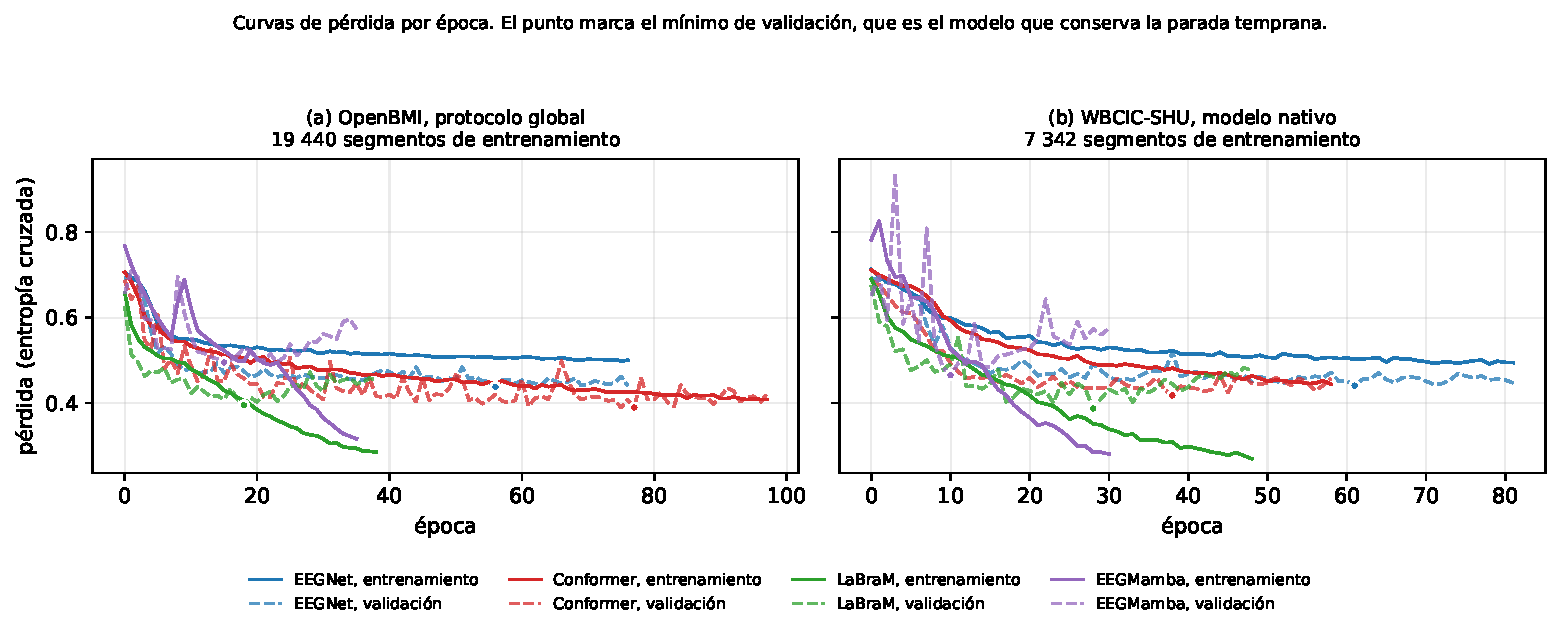
\includegraphics[width=\textwidth]{curvas_perdida.pdf}
\caption{Pérdida de entrenamiento (línea continua) y de validación (discontinua) por época.
(a) \openbmi{}, protocolo global sobre 54 sujetos. (b) WBCIC-SHU, modelo nativo sobre 51
sujetos, con menos de la mitad de segmentos de entrenamiento. El punto marca el mínimo de
validación, que es el modelo que conserva la parada temprana; las épocas posteriores no
forman parte del modelo evaluado.}
\label{fig:curvas}
\end{figure}

En LaBraM y EEGMamba la pérdida de entrenamiento queda por debajo de la de validación sin que esta última
mejore. El orden no sigue el número de parámetros (EEGMamba, con $3.4$ millones, se separa más que LaBraM,
con $5.8$). Los mínimos de validación del panel (a) se sitúan entre $0.39$ y $0.50$. Del panel (a) al (b)
el mínimo se alcanza antes en el Conformer y en EEGMamba, y la oscilación de la validación aumenta en tres de
las cuatro arquitecturas, de forma marcada en EEGMamba. Dos curvas de un único modelo por conjunto no bastan
para atribuir al volumen de datos la parada en las primeras épocas del protocolo intra-sujeto
(subsección~\ref{sec:seleccion-intra}).

\subsection{Referencias externas disponibles}

No hay cifras publicadas de clasificación entre sujetos sobre WBCIC-SHU con las que contrastar estos
resultados. Los autores del conjunto reportan, con validación cruzada de 10 \textit{folds} por sesión,
$0.853$ con \eegnet{} (media de las $153$ sesiones) y $0.818$ en la primera sesión \cite{yang2025wbcic}.
Aunque el protocolo difiere, el modelo nativo obtenido aquí, entre $0.766$ y $0.822$, es coherente con la
cifra de la primera sesión pese a entrenar con menos datos por persona.


\section{Prueba 4: criterios adicionales al desempeño}
\subsection{Descripción} Se examinaron la equivalencia práctica, el costo, la estabilidad, la robustez y la interpretabilidad para complementar la exactitud. La hipótesis de equivalencia se evaluó con un margen de 0.03, sin interpretar la ausencia de significación como equivalencia.
\subsection{Procedimiento} Se aplicó la prueba bayesiana de rangos con signo sobre las medias por sujeto de las semillas 2026, 2027 y 2028, y se comparó con TOST; el detalle y las condiciones de cómputo se presentan en la sección~\ref{sec:estadistica}. La robustez y la saliencia se evaluaron con los pesos de 44 sujetos sobre los 10 apartados, con la semilla 2026. EEGMamba se excluyó de ambos análisis por no estar disponible \texttt{mamba\_ssm} en el entorno de inferencia.
\subsection{Resultados y análisis}
\begin{table}[htbp]\centering\small
\caption{Exactitud \loso{}: probabilidades posteriores para 54 sujetos y media de tres semillas. A y B siguen el orden del par; una decisión requiere probabilidad al menos 0.95.}
\resizebox{\textwidth}{!}{%
\begin{tabular}{lllll}
\toprule
Par A--B & P(A mejor) & P(equivalentes) & P(B mejor) & Decisión \\
\midrule
eegnet-conformer & 0.000 & 1.000 & 0.000 & equivalentes \\
eegnet-labram & 0.000 & 1.000 & 0.000 & equivalentes \\
conformer-labram & 0.000 & 0.999 & 0.001 & equivalentes \\
eegnet-eegmamba & 0.980 & 0.020 & 0.000 & A mejor \\
conformer-eegmamba & 0.864 & 0.136 & 0.000 & indeciso \\
labram-eegmamba & 0.983 & 0.017 & 0.000 & A mejor \\
\bottomrule\end{tabular}}\end{table}
\begin{table}[htbp]\centering\small
\caption{Exactitud intra-sujeto: probabilidades posteriores para 54 sujetos y media de tres semillas. A y B siguen el orden del par; una decisión requiere probabilidad al menos 0.95.}
\resizebox{\textwidth}{!}{%
\begin{tabular}{lllll}
\toprule
Par A--B & P(A mejor) & P(equivalentes) & P(B mejor) & Decisión \\
\midrule
eegnet-conformer & 0.811 & 0.189 & 0.000 & indeciso \\
eegnet-labram & 0.129 & 0.012 & 0.858 & indeciso \\
conformer-labram & 0.000 & 0.011 & 0.989 & B mejor \\
eegnet-eegmamba & 1.000 & 0.000 & 0.000 & A mejor \\
conformer-eegmamba & 0.310 & 0.690 & 0.000 & indeciso \\
labram-eegmamba & 0.999 & 0.001 & 0.000 & A mejor \\
\bottomrule\end{tabular}}\end{table}
\begin{table}[htbp]\centering\small
\caption{Degradación vistos menos no vistos: probabilidades posteriores para 54 sujetos y media de tres semillas. A y B siguen el orden del par; una decisión requiere probabilidad al menos 0.95.}
\resizebox{\textwidth}{!}{%
\begin{tabular}{lllll}
\toprule
Par A--B & P(A mejor) & P(equivalentes) & P(B mejor) & Decisión \\
\midrule
eegnet-conformer & 0.000 & 1.000 & 0.000 & equivalentes \\
eegnet-labram & 0.028 & 0.972 & 0.000 & equivalentes \\
conformer-labram & 0.006 & 0.994 & 0.000 & equivalentes \\
eegnet-eegmamba & 0.000 & 1.000 & 0.000 & equivalentes \\
conformer-eegmamba & 0.000 & 0.999 & 0.001 & equivalentes \\
labram-eegmamba & 0.000 & 0.998 & 0.002 & equivalentes \\
\bottomrule\end{tabular}}\end{table}
En degradación, una caída menor se consideró mejor. Los márgenes 0.01 y 0.02 modificaron las decisiones, por lo que la equivalencia depende del margen elegido. La comparación con TOST se presenta en la sección~\ref{sec:comparacion}.

Para la degradación, con 54 sujetos y media de tres semillas, TOST de Wilcoxon con Holm declaró equivalencia en los seis pares para el margen 0.03, en concordancia con la prueba bayesiana. Para \eegnet{}--LaBraM, la diferencia media fue $-0.021$, el intervalo percentil de remuestreo del 90\% fue $[-0.031, -0.012]$ y $p$ ajustado fue $0.026$; este intervalo rebasa el margen, aunque TOST declara equivalencia. Con ROPE 0.01 ningún par alcanzó probabilidad de equivalencia de 0.95; con ROPE 0.02 solo \eegnet{}--Conformer la alcanzó ($0.981$).
\begin{table}[htbp]\centering\small
\caption{Costo de inferencia con 62 canales. Latencias medianas en ms para lote 1; memoria pico CUDA en MB para lote 64. El contador cubre las operaciones compatibles.}
\resizebox{\textwidth}{!}{%
\begin{tabular}{lllllll}
\toprule
Arquitectura & Parámetros & FLOP/ensayo & CPU & CUDA & Memoria & Tamaño MB \\
\midrule
eegnet & 2898 & 52715968 & 2.09 & 0.67 & 218.25 & 0.07 \\
conformer & 710146 & 262463072 & 7.56 & 8.59 & 1019.07 & 8.37 \\
labram & 5818138 & 3469940000 & 34.04 & 10.61 & 477.61 & 70.20 \\
eegmamba & 3376445 & -- & -- & -- & -- & 40.40 \\
\bottomrule\end{tabular}}\end{table}
Para EEGMamba se informó el número de parámetros; las demás mediciones no estuvieron disponibles por la dependencia \texttt{mamba\_ssm}.
\begin{table}[htbp]\centering\small
\caption{Horas de entrenamiento: suma por ejecución, no tiempo de pared.}
\resizebox{\textwidth}{!}{%
\begin{tabular}{lllll}
\toprule
Arquitectura & Protocolo & Semilla & GPU & Horas \\
\midrule
eegnet & intra & 2026 & A40 & 1.31 \\
eegnet & intra & 2027 & A40 & 1.28 \\
eegnet & intra & 2028 & A40 & 1.26 \\
eegnet & \loso{} & 2026 & A40 & 6.69 \\
eegnet & \loso{} & 2027 & L40S & 6.62 \\
eegnet & \loso{} & 2028 & L40S & 7.26 \\
conformer & intra & 2026 & A40 & 1.37 \\
conformer & intra & 2027 & A40 & 1.38 \\
conformer & intra & 2028 & A40 & 1.36 \\
conformer & \loso{} & 2026 & A40 & 6.14 \\
conformer & \loso{} & 2027 & L40S & 8.52 \\
conformer & \loso{} & 2028 & L40S & 8.90 \\
labram & intra & 2026 & A40 & 6.67 \\
labram & intra & 2027 & L40S & 18.86 \\
labram & intra & 2028 & L40S & 18.96 \\
labram & \loso{} & 2026 & A40 & 21.30 \\
labram & \loso{} & 2027 & L40S & 34.47 \\
labram & \loso{} & 2028 & L40S & 34.22 \\
eegmamba & intra & 2026 & A40 & 10.99 \\
eegmamba & intra & 2027 & L40S & 5.05 \\
eegmamba & intra & 2028 & L40S & 4.93 \\
eegmamba & \loso{} & 2026 & A40 & 24.98 \\
eegmamba & \loso{} & 2027 & L40S & 16.84 \\
eegmamba & \loso{} & 2028 & L40S & 16.65 \\
\bottomrule\end{tabular}}\end{table}
\begin{table}[htbp]\centering\small
\caption{Estabilidad sobre 54 sujetos: desviación entre medias de semilla, tau de Kendall y porcentaje de signo consistente frente a EEGNet.}
\resizebox{\textwidth}{!}{%
\begin{tabular}{llllll}
\toprule
Protocolo & Arquitectura & Semillas & DE & Tau & Signo (\%) \\
\midrule
within & eegnet & 2026-2027-2028 & 0.004 & 0.767 & -- \\
within & eegnet & 2027-2028 & 0.006 & 0.746 & -- \\
within & conformer & 2026-2027-2028 & 0.004 & 0.769 & 68.52 \\
within & conformer & 2027-2028 & 0.000 & 0.757 & 79.63 \\
within & labram & 2026-2027-2028 & 0.001 & 0.833 & 79.63 \\
within & labram & 2027-2028 & 0.001 & 0.842 & 81.48 \\
within & eegmamba & 2026-2027-2028 & 0.006 & 0.547 & 75.93 \\
within & eegmamba & 2027-2028 & 0.005 & 0.589 & 85.19 \\
loso & eegnet & 2026-2027-2028 & 0.002 & 0.836 & -- \\
loso & eegnet & 2027-2028 & 0.000 & 0.816 & -- \\
loso & conformer & 2026-2027-2028 & 0.004 & 0.786 & 50.00 \\
loso & conformer & 2027-2028 & 0.000 & 0.756 & 66.67 \\
loso & labram & 2026-2027-2028 & 0.002 & 0.786 & 40.74 \\
loso & labram & 2027-2028 & 0.003 & 0.797 & 66.67 \\
loso & eegmamba & 2026-2027-2028 & 0.001 & 0.819 & 64.81 \\
loso & eegmamba & 2027-2028 & 0.001 & 0.814 & 74.07 \\
\bottomrule\end{tabular}}\end{table}
\begin{table}[htbp]\centering\small
\caption{Caída de exactitud e intervalo del 95\% ante perturbaciones; 10 sujetos apartados y semilla 2026.}
\resizebox{\textwidth}{!}{%
\begin{tabular}{lllll}
\toprule
Arquitectura & Perturbación & Nivel & Caída & IC 95\% \\
\midrule
conformer & canales & 0.10 & 0.036 & [0.021, 0.053] \\
conformer & canales & 0.20 & 0.068 & [0.042, 0.097] \\
conformer & canales & 0.30 & 0.103 & [0.066, 0.141] \\
conformer & desplazamiento\_s & 0.10 & 0.000 & [-0.005, 0.006] \\
conformer & desplazamiento\_s & 0.25 & 0.023 & [0.011, 0.033] \\
conformer & desplazamiento\_s & 0.50 & 0.053 & [0.030, 0.076] \\
conformer & escala & 0.50 & 0.039 & [0.007, 0.072] \\
conformer & escala & 2.00 & -0.004 & [-0.018, 0.009] \\
conformer & red & 0.10 & -0.000 & [-0.001, 0.001] \\
conformer & red & 0.50 & -0.003 & [-0.008, 0.001] \\
conformer & ruido\_db & 0.00 & 0.064 & [0.045, 0.084] \\
conformer & ruido\_db & 5.00 & 0.019 & [0.006, 0.031] \\
conformer & ruido\_db & 10.00 & 0.000 & [-0.006, 0.007] \\
conformer & ruido\_db & 20.00 & -0.002 & [-0.005, 0.000] \\
eegnet & canales & 0.10 & 0.047 & [0.028, 0.067] \\
eegnet & canales & 0.20 & 0.081 & [0.050, 0.114] \\
eegnet & canales & 0.30 & 0.118 & [0.082, 0.157] \\
eegnet & desplazamiento\_s & 0.10 & 0.009 & [-0.000, 0.021] \\
eegnet & desplazamiento\_s & 0.25 & 0.047 & [0.025, 0.071] \\
eegnet & desplazamiento\_s & 0.50 & 0.080 & [0.048, 0.113] \\
eegnet & escala & 0.50 & 0.013 & [-0.010, 0.038] \\
eegnet & escala & 2.00 & 0.019 & [0.002, 0.036] \\
eegnet & red & 0.10 & 0.000 & [-0.001, 0.002] \\
eegnet & red & 0.50 & 0.005 & [-0.002, 0.012] \\
eegnet & ruido\_db & 0.00 & 0.071 & [0.049, 0.094] \\
eegnet & ruido\_db & 5.00 & 0.030 & [0.017, 0.044] \\
eegnet & ruido\_db & 10.00 & 0.012 & [0.004, 0.020] \\
eegnet & ruido\_db & 20.00 & 0.002 & [-0.001, 0.005] \\
labram & canales & 0.10 & 0.017 & [0.009, 0.025] \\
labram & canales & 0.20 & 0.042 & [0.027, 0.059] \\
labram & canales & 0.30 & 0.070 & [0.047, 0.093] \\
labram & desplazamiento\_s & 0.10 & 0.008 & [-0.002, 0.018] \\
labram & desplazamiento\_s & 0.25 & 0.035 & [0.021, 0.048] \\
labram & desplazamiento\_s & 0.50 & 0.082 & [0.053, 0.111] \\
labram & escala & 0.50 & 0.003 & [-0.002, 0.007] \\
labram & escala & 2.00 & -0.001 & [-0.004, 0.003] \\
labram & red & 0.10 & 0.001 & [-0.000, 0.002] \\
labram & red & 0.50 & 0.002 & [-0.001, 0.006] \\
labram & ruido\_db & 0.00 & 0.076 & [0.054, 0.097] \\
labram & ruido\_db & 5.00 & 0.038 & [0.026, 0.051] \\
labram & ruido\_db & 10.00 & 0.014 & [0.006, 0.024] \\
labram & ruido\_db & 20.00 & 0.002 & [-0.002, 0.008] \\
\bottomrule\end{tabular}}\end{table}
\begin{table}[htbp]\centering\small
\caption{Índices de lateralización para 10 sujetos apartados y semilla 2026.}
\resizebox{\textwidth}{!}{%
\begin{tabular}{llll}
\toprule
Arquitectura & Clase & C3/C4 & Vecindad \\
\midrule
eegnet & izquierda & -0.086 & 0.045 \\
eegnet & derecha & -0.001 & 0.127 \\
conformer & izquierda & -0.005 & 0.065 \\
conformer & derecha & -0.021 & 0.077 \\
labram & izquierda & -0.004 & -0.006 \\
labram & derecha & 0.067 & 0.061 \\
\bottomrule\end{tabular}}\end{table}
No se observó un patrón contralateral uniforme. Los mapas describen sensibilidad de los modelos y no establecen causalidad. La eficiencia de datos se examinó mediante la calibración de la subsección~\ref{sec:fewshot}.
\begin{figure}[htbp]\centering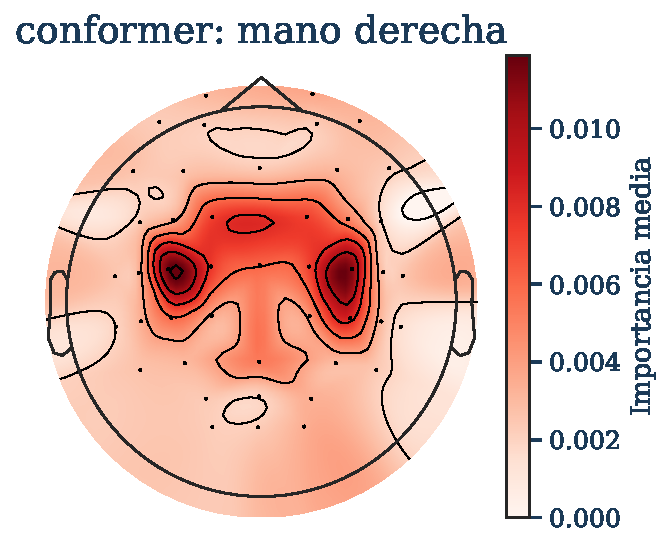
\includegraphics[width=0.65\textwidth]{figuras/interp_conformer_derecha.pdf}\caption{Sensibilidad espacial o filtros: interp conformer derecha; 10 sujetos apartados, semilla 2026.}\end{figure}
\begin{figure}[htbp]\centering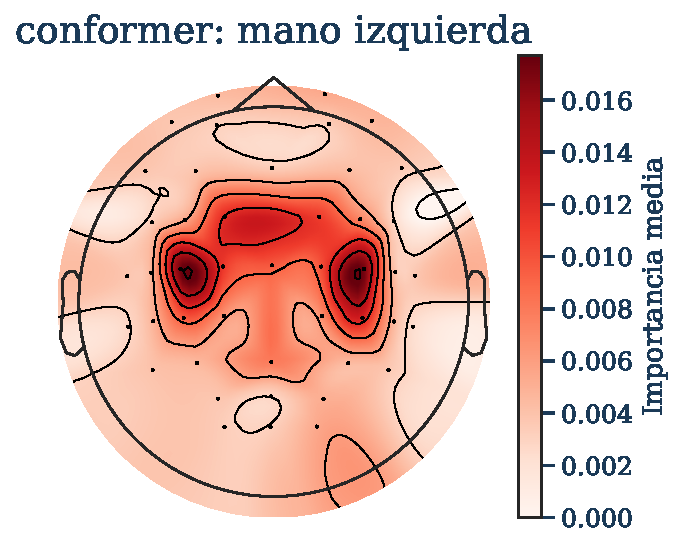
\includegraphics[width=0.65\textwidth]{figuras/interp_conformer_izquierda.pdf}\caption{Sensibilidad espacial o filtros: interp conformer izquierda; 10 sujetos apartados, semilla 2026.}\end{figure}
\begin{figure}[htbp]\centering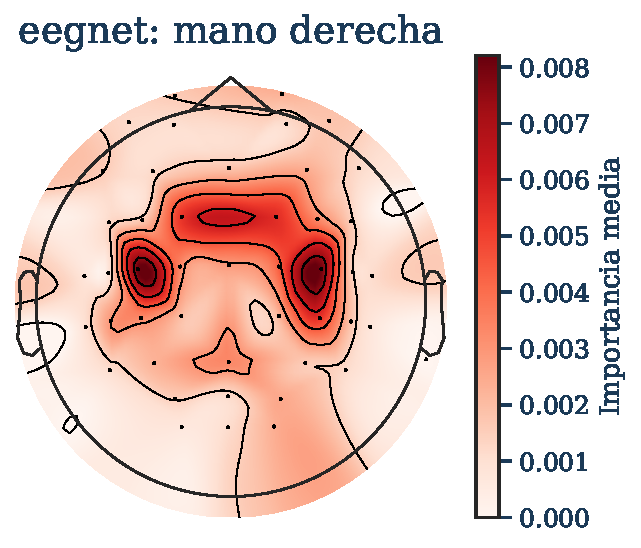
\includegraphics[width=0.65\textwidth]{figuras/interp_eegnet_derecha.pdf}\caption{Sensibilidad espacial o filtros: interp eegnet derecha; 10 sujetos apartados, semilla 2026.}\end{figure}
\begin{figure}[htbp]\centering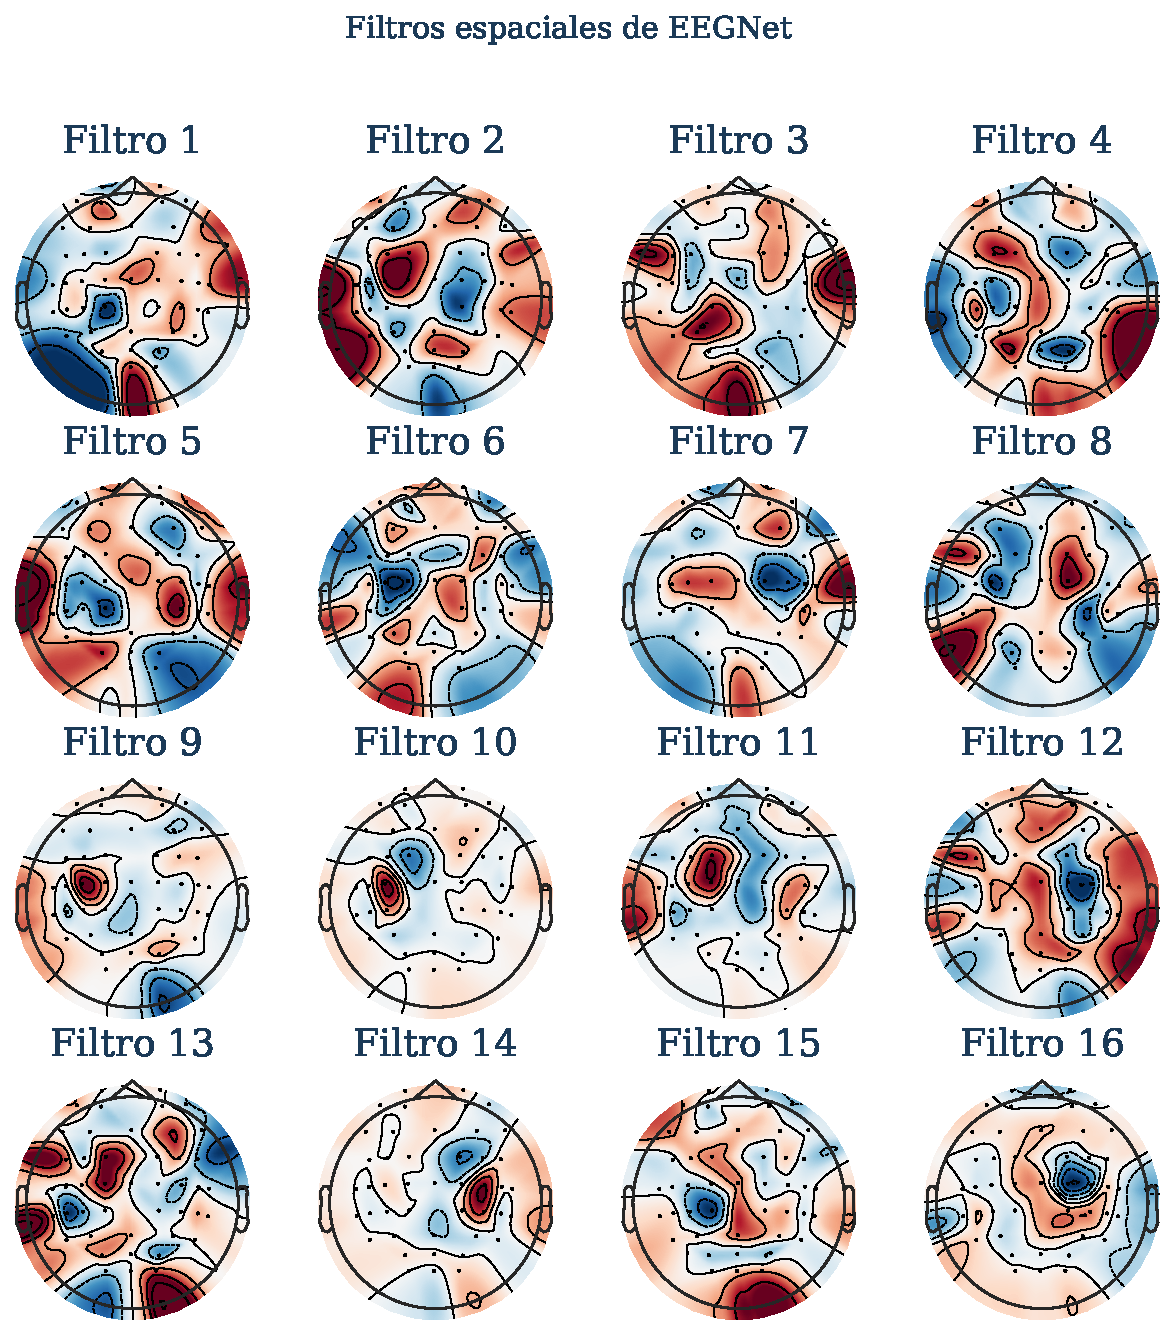
\includegraphics[width=0.65\textwidth]{figuras/interp_eegnet_filtros.pdf}\caption{Sensibilidad espacial o filtros: interp eegnet filtros; 10 sujetos apartados, semilla 2026.}\end{figure}
\begin{figure}[htbp]\centering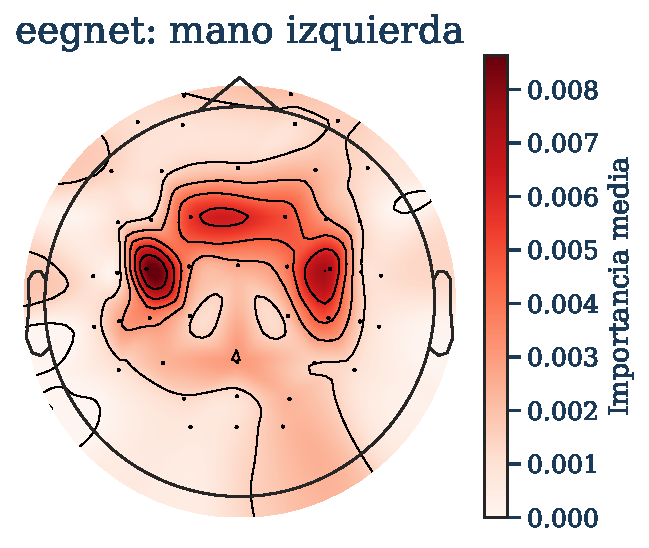
\includegraphics[width=0.65\textwidth]{figuras/interp_eegnet_izquierda.pdf}\caption{Sensibilidad espacial o filtros: interp eegnet izquierda; 10 sujetos apartados, semilla 2026.}\end{figure}
\begin{figure}[htbp]\centering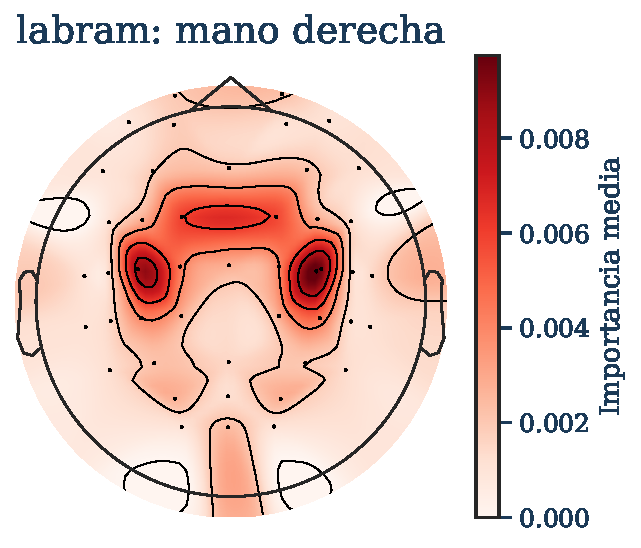
\includegraphics[width=0.65\textwidth]{figuras/interp_labram_derecha.pdf}\caption{Sensibilidad espacial o filtros: interp labram derecha; 10 sujetos apartados, semilla 2026.}\end{figure}
\begin{figure}[htbp]\centering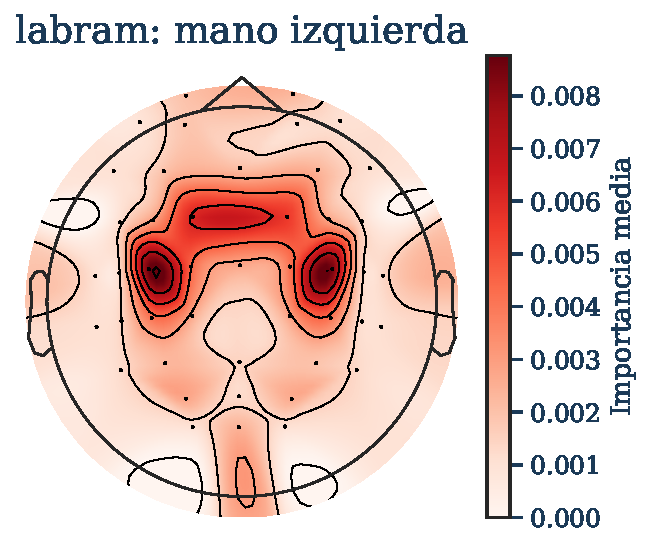
\includegraphics[width=0.65\textwidth]{figuras/interp_labram_izquierda.pdf}\caption{Sensibilidad espacial o filtros: interp labram izquierda; 10 sujetos apartados, semilla 2026.}\end{figure}

\section{Análisis comparativo y discusión}

\subsection{Especificaciones previstas frente a obtenidas}

La tabla~\ref{tab:especificaciones} contrasta las especificaciones del anteproyecto con las condiciones evaluadas.
\begin{table}[H]
\centering
\caption{Especificaciones previstas y obtenidas.}
\label{tab:especificaciones}
\small
\begin{tabular}{p{2.8cm}p{3.2cm}p{5.2cm}p{2cm}}
\toprule
\textbf{Requisito} & \textbf{Previsto} & \textbf{Obtenido} & \textbf{Sección} \\
\midrule
Datos multisujeto & Conjunto público multisujeto & \openbmi{}: 54 sujetos; WBCIC-SHU: 51 sujetos & \ref{sec:fase1} \\
Preprocesamiento reproducible & Flujo unificado & Flujo común para las arquitecturas & \ref{sec:fase2} \\
Arquitecturas & Conformer, Mamba y modelo fundacional & Conformer, EEGMamba y LaBraM; \eegnet{} como línea base & \ref{cap:metodologia-modelos} \\
Configuraciones & Monousuario y multiusuario & Intra-sujeto por sesión y \loso{} & \ref{sec:fase4} \\
Evaluación y métricas & Protocolo comparativo con métricas & Exactitud, kappa, \dsi{}, \idp{}, Wilcoxon con Holm, TOST, bootstrap y prueba bayesiana & \ref{sec:fase4} \\
Prueba estadística & Friedman con post-hoc & Contrastes pareados con Holm, equivalencia e incertidumbre; la justificación se expone en el capítulo 2 & \ref{sec:fase4} \\
Validación externa & No prevista & Sí, con WBCIC-SHU & \ref{sec:protocolos-extra} \\
\bottomrule
\end{tabular}
\end{table}

\textbf{Indicador de degradación.} Sobre \openbmi{}, el indicador clásico
(ecuación~\eqref{eq:dsi-clasico}) resulta negativo, compatible con que lo dominen el volumen de datos y el
procedimiento de evaluación, mientras que la formulación propuesta (ecuación~\eqref{eq:dsi}) separa la
pertenencia del participante al entrenamiento del volumen de datos. Es positivo en las cuatro arquitecturas y
solo en LaBraM alcanza significación tras Holm (subsección~\ref{sec:dsi-resultados}).

\textbf{Degradación ante el cambio de protocolo de adquisición.} Al aplicar un mismo conjunto de pesos a un
conjunto registrado en otra institución, con otro amplificador y otro montaje, la exactitud cae entre $0.095$
y $0.123$ respecto de personas nuevas del conjunto de origen, con intervalos que excluyen el cero en las
cuatro arquitecturas (sección~\ref{cap:validacion-externa}). La degradación ante personas nuevas del mismo
conjunto es menor en estimación puntual ($0.020$ a $0.041$ en \loso{} y $0.055$ a $0.087$ con sujetos
apartados), pero con $10$ sujetos apartados la diferencia entre ambas caídas no alcanza significación. Lo que
queda establecido es que la generalización observada dentro de \openbmi{} no se mantiene sin pérdida al
cambiar de conjunto de datos; que el cambio de protocolo degrade más que el de persona es compatible con los
datos, pero el diseño no lo establece. No se debe a que el segundo conjunto sea más difícil (un modelo
entrenado sobre él alcanza entre $0.766$ y $0.822$) ni, bajo el contraste de normalización, a una diferencia
de escala de amplitud entre equipos.

\textbf{Participantes de bajo rendimiento.} El fenómeno de bajo rendimiento en imaginación motora se atribuye
a propiedades de la señal del participante y no a la capacidad del modelo para generalizar
\cite{vidaurre2010,blankertz2010}, por lo que se examina con el protocolo \textbf{intra-sujeto}. Con el umbral
del $70$\,\% de la sección~\ref{sec:dsi}, quedan por debajo $37$ de los $54$ sujetos con LaBraM, $41$ con
\eegnet{}, $45$ con el Conformer y $49$ con EEGMamba, y \textbf{34 participantes, el $63$\,\%, quedan por
debajo con las cuatro arquitecturas a la vez}, del mismo orden que el $53.7$\,\% reportado para este conjunto
\cite{lee2019}. La cifra tiende a sobrestimar la prevalencia, porque el volumen de entrenamiento ($144$
segmentos) y la selección del modelo con $36$ ensayos (subsección~\ref{sec:seleccion-intra}) actúan en la misma
dirección, y con $20$ ensayos de prueba la clasificación respecto del umbral tiene ruido en ambos sentidos.

La figura~\ref{fig:solapamiento} muestra que las cuatro arquitecturas obtienen baja exactitud en las mismas
personas. Bajo independencia de los fallos, conservando la tasa de cada arquitectura, cabría esperar $21.2$
participantes bajo umbral con las cuatro y $0.1$ por encima con las cuatro; se observan $34$ y $5$. El
resultado se reproduce en las tres semillas ($34$, $33$ y $33$ participantes), y el conjunto concreto es estable
entre semillas en el protocolo intra-sujeto (Jaccard medio de $0.91$ a $0.99$) y menos en \loso{} ($0.66$ y
$0.68$ en el Conformer y LaBraM).

\begin{figure}[H]
\centering
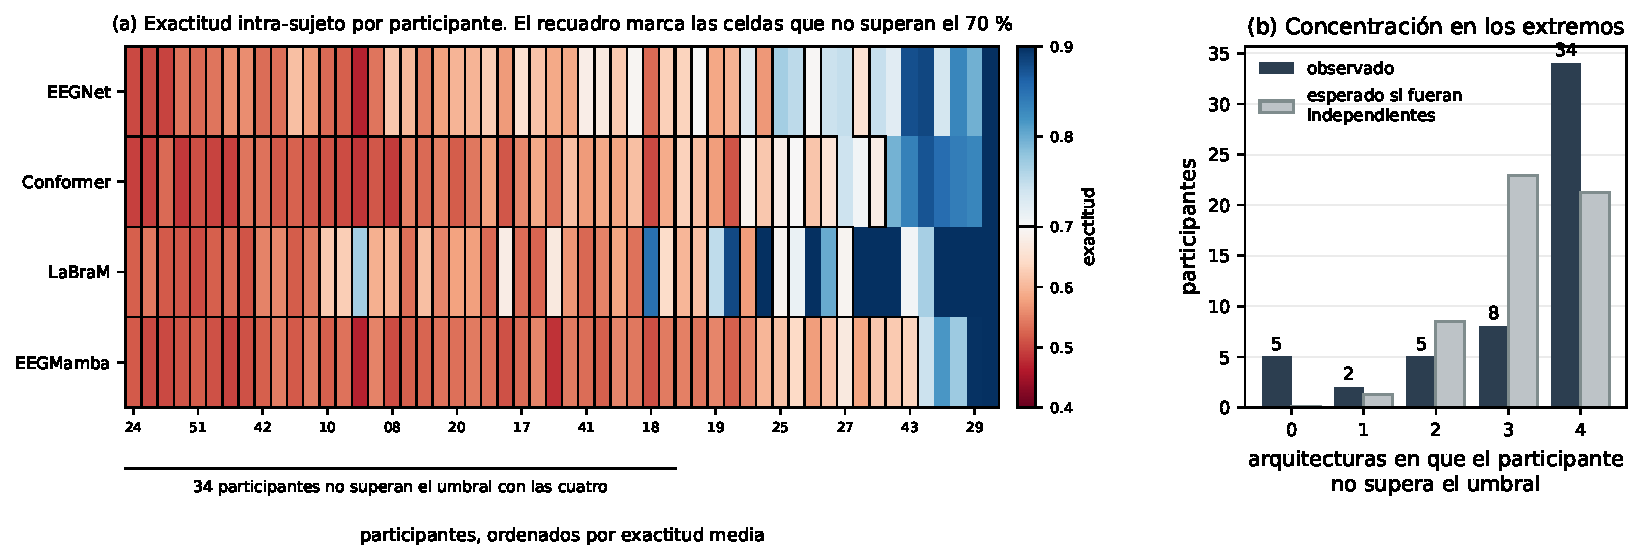
\includegraphics[width=\textwidth]{solapamiento_bajo_rendimiento.pdf}
\caption{Solapamiento de los participantes de bajo rendimiento entre las cuatro
arquitecturas, protocolo intra-sujeto, con la media de tres semillas por participante. (a) Exactitud por participante, ordenados por su
media; el recuadro marca las celdas que no superan el umbral del $70$\,\% y la escala de
color está centrada en ese mismo umbral. (b) Número de arquitecturas en que cada
participante queda bajo umbral, frente a lo esperado si los errores de las cuatro fueran
independientes, conservando sus tasas marginales. Las cuatro arquitecturas comparten las
mismas particiones, de modo que esa referencia describe la magnitud de la coincidencia y
no su causa.}
\label{fig:solapamiento}
\end{figure}

Esta coincidencia admite dos lecturas que los datos no separan: que la dificultad sea una propiedad de la
señal del participante, que afecta por igual a arquitecturas muy distintas, o que proceda de las condiciones
de evaluación que las cuatro comparten (las mismas particiones, con $36$ ensayos de validación y $20$ de
prueba, y el mismo efecto de la selección del modelo). La referencia de independencia cuantifica cuánto se
aparta la coincidencia de la esperada, no su causa; separarlas exigiría particiones distintas por arquitectura
o un conjunto de prueba mayor por participante.

En \loso{} solo $13$ de los $54$ participantes, el $24$\,\%, quedan por debajo del umbral con las cuatro
arquitecturas ($17$, $19$, $15$ y $26$ por arquitectura). Los dos valores \textbf{no estiman la misma
cantidad}: el intra-sujeto mide la exactitud de un modelo entrenado con $144$ segmentos de la persona, y
\loso{} la de un modelo general entrenado con unos $18\,000$ segmentos de otras $51$ personas. La correlación
entre ambas exactitudes por participante va de $0.309$ en el Conformer (intervalo al $95$\,\% que incluye el
cero) y $0.364$ en \eegnet{} a $0.485$ en EEGMamba y $0.679$ en LaBraM, de modo que ser un participante
difícil no significa lo mismo bajo cada protocolo. Una parte de lo que el protocolo intra-sujeto contabiliza
como bajo rendimiento es atribuible al propio protocolo, por la escasez de datos y la selección del modelo;
esto no niega el fenómeno, documentado de forma independiente \cite{vidaurre2010,lee2019}, pero acota su
magnitud y apoya los modelos entrenados entre sujetos.

Hay, por tanto, dos limitaciones de naturaleza distinta. \textbf{La primera es del modelo}: el cambio de
protocolo de adquisición degrada su desempeño de forma clara en las cuatro arquitecturas. \textbf{La segunda se
manifiesta en el usuario}: una parte considerable de los participantes no alcanza el umbral funcional ni
siquiera con un modelo entrenado sobre sí mismos, sin que este protocolo separe qué parte corresponde a la
señal y cuál a las condiciones de evaluación. Reducir la primera, objeto de este trabajo, no resuelve la
segunda.

\textbf{Comparación entre arquitecturas.} \eegnet{}, el Conformer y LaBraM son equivalentes dentro de $\pm 0.03$
en \loso{}, EEGMamba se separa de las tres y en el protocolo intra-sujeto ningún contraste es equivalente.
Las ordenaciones pequeñas no se mantienen entre semillas, porque la variabilidad por inicialización de las
diferencias ($0.001$ a $0.010$) es del orden de las diferencias entre las tres primeras. Esto refuerza la
lectura de que ninguna arquitectura es más robusta: el menor \dsi{} es el de \eegnet{}, el menor \idp{} el de
EEGMamba, el menor recuento bajo umbral el de LaBraM, y ninguna es la mejor en los tres ejes.

\textbf{Preprocesamiento y aumentación.} En el protocolo intra-sujeto, con una semilla, los efectos de la banda,
la ventana y la aumentación difieren entre arquitecturas ($+0.078$ para la banda $\mu+\beta$ en el Conformer y
$+0.042$ para la ventana de \seg{0} a \seg{2} en \eegnet{}) y no pueden leerse como propiedades de la señal:
en \eegnet{} y el Conformer están condicionados al régimen de optimización, y en $21$ de los $22$ contrastes el
signo del efecto coincide con el del cambio en la proporción de particiones que se detienen en el suelo de $30$
épocas. La ventana de \seg{0} a \seg{2} no justifica cambiar la ventana fijada de antemano, pero indica que la
elección de \seg{0} a \seg{4} no es neutra.

\textbf{Alineamiento y calibración.} Con una semilla y de forma transductiva, el alineamiento euclidiano
aumenta la exactitud \loso{} de forma inequívoca solo en EEGMamba ($+0.0463$) y en LaBraM ($+0.0249$); no
cambia de forma detectable la brecha entre vistos y no vistos y no reduce la caída por protocolo, porque eleva
la exactitud en los $10$ sujetos apartados de \openbmi{} y no en WBCIC-SHU (sección~\ref{sec:ea-transferencia}).
La calibración con $10$ a $20$ ensayos no mejoró la exactitud con este procedimiento: las $24$ ganancias medias
fueron negativas y $16$ significativas tras Holm. Eso no establece que la calibración no sirva, porque el
procedimiento reentrena una sola capa con hiperparámetros fijos y evalúa sobre las mismas sesiones. La
aumentación y la calibración no se probaron en la transferencia a WBCIC-SHU, de modo que nada puede afirmarse
sobre su efecto en la degradación por protocolo.

\textbf{El eje de la representación como trabajo futuro.} Las cuatro arquitecturas consumen la señal en el
dominio del tiempo. Pese a diferir hasta en tres órdenes de magnitud en parámetros, con y sin preentrenamiento y
con mecanismos tan distintos como la convolución separable, la atención y los espacios de estados, los modelos de
$44$ sujetos se sitúan entre $0.598$ y $0.623$ sobre WBCIC-SHU (tabla~\ref{tab:descomposicion}) y la caída
atribuible al protocolo se mantiene en menos de tres puntos de rango ($0.095$ a $0.123$). Esto es compatible
con que el límite no dependa de la capacidad de la arquitectura, pero el trabajo no distingue entre la
representación de entrada compartida, el cambio de protocolo (un factor compuesto) y la separabilidad de la
señal de cada participante: la representación es una hipótesis entre varias.

Una vía para contrastarla es un objetivo de predicción en el espacio latente en lugar de la forma de onda.
EEG-JEPA \cite{li2026eegjepa} lo implementa, preentrenado sobre EEG clínico que no incluye \openbmi{} entre sus
fuentes declaradas, y alcanza una exactitud balanceada del $55.38$\,\% en BCI-IV-2a (cuatro clases), frente a
$44.82$\,\% de \eegnet{}, $46.96$\,\% del EEG-Conformer, $48.69$\,\% de LaBraM-Base y $51.38$\,\% de una línea
base de reconstrucción, con cifras de líneas base tomadas de trabajos previos y no de un reentrenamiento común.
Corresponden a otro conjunto y protocolo y no miden el comportamiento ante un cambio de protocolo de
adquisición, que es lo que contrastaría la hipótesis. No se incorporó porque no se localizaron pesos
preentrenados públicos y su reproducción desde cero excede el alcance de este trabajo; queda como línea de
trabajo futuro, sujeta a una modificación de la metodología.




\textbf{Regla de decisión.} Bajo la regla de la sección~\ref{sec:criterios-adicionales}, fijada después del primer análisis, \eegnet{}, Conformer y LaBraM son equivalentes por pares en exactitud \loso{} y en degradación según la prueba bayesiana y TOST con Holm. \eegnet{} tiene menor costo medido y resulta preferida bajo esta regla, para las semillas y regímenes indicados y una sola base de datos. La comparación no demuestra superioridad universal. La referencia inter-sujeto de \cite{kwon2020} ya se contextualizó en la subsección~\ref{sec:desempeno-global}.

\section{Alcances y limitaciones}
\label{sec:limitaciones}

Las limitaciones siguientes condicionan la interpretación de los resultados; los análisis sin corrección
por comparaciones múltiples son exploratorios.

\begin{itemize}
  \item \textbf{Cambio de régimen entre semillas.} Las bases del primer régimen de \eegnet{}, el Conformer y
        LaBraM se entrenaron sin recorte de gradiente, en GPU A40 y con otra versión del código de entrenamiento; las del segundo llevan recorte y GPU L40S. El contraste de cada variante con la base de la
        semilla $2026$ está confundido, en esas tres arquitecturas, con este cambio compuesto. Su cota
        ($0.010$ a $0.020$ de exactitud, tabla~\ref{tab:confusor}) descarta un efecto medio mayor, no uno nulo.
        En el protocolo intra-sujeto de \eegnet{} y del Conformer no existe base con recorte, la cota no es
        estimable y sus $16$ contrastes de ablación se informan como condicionados al régimen; no se
        rehízo esa base por presupuesto de cómputo. No se midió la fracción de pasos de
        optimización en que el recorte actúa. La sección~\ref{sec:tf-entrenamiento} propone un régimen coherente para repetir variantes.
  \item \textbf{Variantes con una sola semilla.} Todas las variantes (ablaciones, alineamiento, reflexión de
        canales) se ejecutaron con la semilla $2026$, por decisión de presupuesto previa a los resultados.
        Su variabilidad por semilla no está incorporada y sus equivalencias valen para esa semilla (el
        desplazamiento medio entre semillas llega a $0.008$ a $0.009$). Lo mismo vale para las variantes con
        alineamiento en la validación externa. La sección~\ref{sec:tf-entrenamiento} propone ampliar las semillas.
  \item \textbf{Ablaciones recortadas en LaBraM y EEGMamba.} En estas dos arquitecturas solo se ejecutaron la
        reflexión de canales, el ruido en Fourier y la ventana de \seg{0} a \seg{2}, por coste de cómputo y
        con decisión previa a los resultados; los efectos de subbanda no se extienden a ellas. La sección~\ref{sec:tf-preprocesamiento} propone ampliar las ablaciones de subbanda.
  \item \textbf{Ruido en Fourier.} La amplitud $\sigma = 0.1$ es una elección propia y no se probaron otras. La sección~\ref{sec:tf-entrenamiento} propone estudiar su sensibilidad.
  \item \textbf{Selección del modelo intra-sujeto.} La parada temprana con $36$ ensayos conserva con
        frecuencia un modelo de las épocas de calentamiento, y en $21$ de los $22$ contrastes de ablación el
        signo del efecto coincide con el del cambio en esa proporción; las diferencias intra-sujeto no se
        atribuyen por tanto a la capacidad ni a la representación. La sección~\ref{sec:tf-entrenamiento} propone selección de parada mediante validación anidada.
  \item \textbf{Tres semillas.} La desviación entre semillas tiene dos grados de libertad y es una estimación
        gruesa; las semillas se emparejan por índice aunque sus inicializaciones son independientes, y los
        \textit{folds} \loso{} se tratan como independientes aunque comparten $49$ de sus $51$ sujetos de
        entrenamiento. Los intervalos por remuestreo de sujetos no incorporan la variabilidad por semilla; el
        jerárquico sí, y es ligeramente conservador. La sección~\ref{sec:tf-entrenamiento} propone ampliar las semillas.
  \item \textbf{Calibración.} Con el procedimiento probado no hubo ganancia; no se ajustaron los
        hiperparámetros, se calibró y evaluó sobre las mismas sesiones (escenario favorable) y no se calibró el
        modelo transferido ni se repitió la ejecución, de modo que no se descarta que otro procedimiento sea
        útil. La sección~\ref{sec:tf-transferencia} propone evaluar calibración prospectiva.
  \item \textbf{Alineamiento euclidiano transductivo.} Estima la covarianza con todos los segmentos sin
        etiqueta del participante de prueba, por lo que sus resultados no son \textit{zero-shot} estricto. La sección~\ref{sec:tf-transferencia} propone alineamiento prospectivo.
  \item \textbf{Diez sujetos apartados, de un solo sorteo.} La caída por persona se estima sobre $10$
        sujetos que rinden entre $2.2$ y $3.1$ puntos menos que el resto en \loso{}; sus intervalos no la
        distinguen de la caída por protocolo y el \idp{} hereda esa imprecisión (amplitud de $0.16$ a $0.21$).
        Además, su columna de sujetos vistos comparte sesión con el entrenamiento, lo que tiende a
        sobrestimar la caída por persona. La sección~\ref{sec:tf-datos} propone repetir las particiones de sujetos apartados.
  \item \textbf{Protocolo de adquisición como factor compuesto.} Las diferencias residuales de
        armonización (tabla~\ref{tab:armonizacion}), la asimetría de volumen entre conjuntos ($144$ segmentos
        por persona en WBCIC-SHU frente a $360$) y la referencia de promedio común calculada sobre conjuntos de
        electrodos distintos forman parte de ese factor y no se separan de él. El \dsi{} y el \idp{} proceden
        de protocolos distintos y sus magnitudes no son comparables entre sí. La sección~\ref{sec:tf-transferencia} propone contrastes entre adquisiciones armonizadas.
  \item \textbf{Modelo nativo y preentrenamiento.} El modelo nativo de WBCIC-SHU vio a los $51$ participantes,
        de modo que su cifra es un límite superior sobre sujetos vistos, y no hay protocolo entre sujetos
        dentro de ese conjunto. La ausencia de WBCIC-SHU en el preentrenamiento de LaBraM se comprobó solo
        frente a las fuentes declaradas por sus autores. La sección~\ref{sec:tf-transferencia} propone validación entre sujetos en el destino.
  \item \textbf{Normalización del destino.} Las políticas por segmento y por sujeto se aplican a un modelo
        entrenado con los estadísticos del origen; el contraste descarta una diferencia de ganancia global
        como explicación de la caída, no cualquier diferencia de escala. La sección~\ref{sec:tf-transferencia} propone evaluar protocolos armonizados.
  \item \textbf{Reserva vista y artefactos residuales.} El conjunto visto del \dsi{} comparte sesión con el
        entrenamiento. Cuatro sujetos quedan marcados por el control ocular tras la limpieza; su efecto se
        acota (subsección~\ref{sec:sensibilidad}), pero no se elimina. La sección~\ref{sec:tf-datos} propone ampliar las particiones independientes por participante.
\end{itemize}

% =====================================================================
%  DECISIONES
% =====================================================================


La ausencia de una búsqueda sistemática de hiperparámetros por arquitectura pudo afectar el orden relativo de desempeño. El indicador de degradación entre protocolos dependió de un único sorteo de sujetos apartados. La robustez y la interpretabilidad se limitaron a una semilla y excluyeron EEGMamba por la dependencia no disponible. La regla de decisión se fijó después del primer análisis y debe interpretarse como exploratoria. La ampliación de particiones, modelos y evaluación se plantea en el capítulo~\ref{cap:trabajos-futuros}.

\section{Conclusiones}

\begin{itemize}
\item En \openbmi{}, la comparación de protocolos y el indicador de degradación mostraron que la diferencia entre personas vistas y no vistas debe distinguirse del cambio de volumen de datos; solo LaBraM mostró degradación significativa tras Holm.
\item Las variantes de procesamiento y alineamiento no tuvieron un efecto común a todas las arquitecturas; la calibración ensayada con pocos ejemplos no produjo ganancia.
\item La transferencia a WBCIC-SHU redujo la exactitud respecto de personas nuevas de \openbmi{}, lo que limita la extrapolación entre protocolos de adquisición.
\item Los criterios adicionales mostraron que la elección de arquitectura depende tanto de la equivalencia práctica como del costo y de las condiciones de medición; la robustez y la saliencia se examinaron en una sola partición y semilla.
\end{itemize}

